% Nafs-Aql Technical Specification. Build: ../../tools/tectonic nafs_aql_spec.tex
\documentclass[11pt,a4paper]{article}
\usepackage[margin=2.2cm]{geometry}
\usepackage[utf8]{inputenc}\usepackage[T1]{fontenc}
\usepackage{amsmath,amssymb,amsthm}
\usepackage{booktabs,array,longtable,multirow}
\usepackage{graphicx,xcolor}
\usepackage{tikz,pgfplots}\pgfplotsset{compat=1.18}
\usetikzlibrary{arrows.meta,positioning,shapes.geometric,fit,calc,backgrounds}
\usepackage{enumitem}\setlist{nosep,leftmargin=*}
\usepackage{listings}
\usepackage{microtype}
\usepackage{url}
\usepackage[hidelinks,pdfauthor={Dirac R\&D Team}]{hyperref}
\usepackage{fancyhdr}
% Shared palette, TikZ styles and macros for all Nafs-Aql documents
\definecolor{navy}{HTML}{1F3A5F}
\definecolor{teal}{HTML}{1B8A8F}
\definecolor{amber}{HTML}{C97D10}
\definecolor{crimson}{HTML}{B3263E}
\definecolor{violet}{HTML}{6A4C9C}
\definecolor{leaf}{HTML}{3A8F4B}
\definecolor{slate}{HTML}{5B6770}
\definecolor{sand}{HTML}{F4EFE6}
\tikzset{
  blk/.style={rounded corners=2.5pt,draw=#1!85!black,fill=#1!12,thick,align=center,
              font=\scriptsize,inner sep=3pt,minimum height=0.72cm},
  blk/.default=navy,
  sblk/.style={rounded corners=2.5pt,draw=#1!85!black,fill=#1!12,thick,align=center,
              font=\tiny,inner sep=2pt,minimum height=0.55cm},
  sblk/.default=navy,
  dm/.style={diamond,aspect=2.2,draw=amber!85!black,fill=amber!15,thick,font=\tiny,
             align=center,inner sep=0.5pt},
  st/.style={circle,draw=#1!85!black,fill=#1!15,thick,font=\scriptsize,minimum size=0.78cm,inner sep=0pt},
  st/.default=navy,
  arr/.style={-{Stealth[length=4pt,width=3pt]},thick,draw=slate},
  dsh/.style={-{Stealth[length=4pt,width=3pt]},thick,dashed,draw=slate!80},
  lab/.style={font=\tiny,fill=white,inner sep=1pt,text=black!80},
  grp/.style={rounded corners=4pt,draw=#1!60,dashed,thick,inner sep=5pt,fill=#1!4},
  grp/.default=slate,
  grplab/.style={font=\tiny\bfseries,text=#1!80!black,anchor=north west,inner sep=2pt},
  grplab/.default=slate
}
\pgfplotsset{every axis/.append style={font=\scriptsize,grid=major,grid style={black!10},
  legend style={font=\tiny,draw=none,fill=white,fill opacity=.85,text opacity=1},
  tick label style={font=\tiny},label style={font=\scriptsize}}}
% ---- shared names (single source of truth) ----
\newcommand{\Sys}{Nafs-Aql}
\newcommand{\Sone}{System~1}
\newcommand{\Stwo}{System~2}
\newcommand{\Gate}{Aql Gate}
\newcommand{\Hub}{Verifier Hub}
\newcommand{\Ledger}{Muhasaba Ledger}
\newcommand{\Distil}{Tazkiya Distillation}
\newcommand{\Mem}{Context Manager}
\newcommand{\Gw}{Rust Gateway}
\newcommand{\Harness}{Eval Harness}

\newcommand{\TasksPhaseA}{
\begin{tabular}{@{}p{1.1cm}p{2.3cm}p{6.0cm}p{0.9cm}p{1.9cm}p{1.7cm}@{}}
\toprule ID & Epic & Task & PW & Depends & MoSCoW\\\midrule
P0-T01 & E0.1 Environment & Build llama.cpp and vLLM-CPU container; publish serving recipes for Profile A & 1.0 & -- & Must\\
P0-T02 & E0.1 Environment & Pin model revisions, GGUF hashes, chat-template hashes; write model manifest & 0.5 & P0-T01 & Must\\
P0-T03 & E0.2 Measurement & Implement minimal Eval Harness (dataset loaders, exact verifiers for GSM8K/HumanEval/schema, metrics) & 2.0 & P0-T01 & Must\\
P0-T04 & E0.2 Measurement & Run fast-only and slow-only baselines on $\ge$ 4600 tasks; fit q, (r,phi), e1(s), e2(s), cost ratio, discordance & 1.5 & P0-T03 & Must\\
P0-T05 & E0.2 Measurement & Measure accuracy vs thinking budget per domain (H4) and acceptance-rate distribution & 1.0 & P0-T04 & Must\\
P0-T06 & E0.3 Hybrid gate & llama-bench Qwen3.5-2B/4B vs Qwen3-1.7B/4B on target CPU (H7); decide Profile C & 0.5 & P0-T01 & Must\\
P0-T07 & E0.4 Workspace & Create Cargo workspace, CI (fmt, clippy, test on Linux and macOS), config schema & 1.0 & -- & Must\\
\bottomrule\end{tabular}}
\newcommand{\TasksPhaseB}{
\begin{tabular}{@{}p{1.1cm}p{2.3cm}p{6.0cm}p{0.9cm}p{1.9cm}p{1.7cm}@{}}
\toprule ID & Epic & Task & PW & Depends & MoSCoW\\\midrule
P1-T01 & E1.1 Gateway & axum gateway: /v1/chat, /v1/chat/stream (SSE), auth, rate limit, metrics, OpenAPI at /openapi.json & 2.0 & P0-T07 & Must\\
P1-T02 & E1.2 Backends & Backend trait + llama-server and vLLM implementations: logprobs, parallel samples, thinking toggle, retry, semaphore & 2.0 & P0-T07 & Must\\
P1-T03 & E1.3 Orchestrator & Trace-state automaton with fixed-rule gate, budget forcing, caps, decision record, assurance levels & 2.5 & P1-T02 & Must\\
P1-T04 & E1.4 Verifiers & Verifier Hub v1: code sandbox (subprocess limits), JSON Schema verifier & 2.0 & P0-T07 & Must\\
P1-T05 & E1.5 Memory & SQLite conversation store, JSONL traces, context cap and prompt-cache prefix preservation & 1.5 & P0-T07 & Must\\
P1-T06 & E1.6 Web UI & Chat room UI (askama + htmx + WebSocket), reasoning mode and assurance badges, controller event stream & 2.0 & P1-T01 & Must\\
P1-T07 & E1.7 MVP acceptance & Profile selection, MVP acceptance tests, latency targets measured on reference machine & 1.0 & P1-T03, P1-T04, P1-T05, P1-T06 & Must\\
\bottomrule\end{tabular}}
\newcommand{\TasksPhaseC}{
\begin{tabular}{@{}p{1.1cm}p{2.3cm}p{6.0cm}p{0.9cm}p{1.9cm}p{1.7cm}@{}}
\toprule ID & Epic & Task & PW & Depends & MoSCoW\\\midrule
P2-T01 & E2.1 Calibrated gate & Feature extraction, logistic/isotonic estimator, cost-ratio rule, budget mode, recalibration job & 2.5 & P0-T04, P1-T03 & Must\\
P2-T02 & E2.2 Verified loop & Sequential verified sampling, evidence-fed retries, caps from Beta fit, R$\le$1 on non-verifiable & 2.0 & P1-T03, P0-T05 & Must\\
P2-T03 & E2.3 Verifier quality & Math verifier (numeric + SymPy sidecar), mutation-testing harness, (r,phi) publication, judge hard gate & 2.0 & P1-T04 & Must\\
P2-T04 & E2.4 Audit and ledger & 5 percent audit stream, capability table with unmeasured labels, adapter-hash keying & 1.5 & P2-T01 & Must\\
P2-T05 & E2.5 Resilience & Backend reconnect, degraded mode, prompt-injection delimiting & 1.0 & P1-T02 & Must\\
P2-T06 & E2.6 Gate G2 evaluation & Coupling test ($\ge$ 200 trials), calibration test ($\ge$ 2900), 3-point non-inferiority ($\ge$ 700 pairs) & 1.5 & P2-T01, P2-T02, P2-T03 & Must\\
\bottomrule\end{tabular}}
\newcommand{\TasksPhaseD}{
\begin{tabular}{@{}p{1.1cm}p{2.3cm}p{6.0cm}p{0.9cm}p{1.9cm}p{1.7cm}@{}}
\toprule ID & Epic & Task & PW & Depends & MoSCoW\\\midrule
P3-T01 & E3.1 Data pipeline & Dataset builder from verified traces; schema; dedupe; domain cap; abstain and replay mixing; privacy redaction & 1.5 & P2-T04 & Must\\
P3-T02 & E3.2 Synthetic data & System 2 synthetic generation on benchmark-like prompts with held-out verifier & 1.0 & P3-T01 & Should\\
P3-T03 & E3.3 Unsloth training & Unsloth LoRA scripts, GPU runbook (T4), checkpoint and adapter hashing, GGUF export & 1.5 & P3-T01 & Must\\
P3-T04 & E3.4 Promotion & Promotion gate with confidence bounds, regression suite, human sign-off, one-command rollback & 1.5 & P3-T03 & Must\\
\bottomrule\end{tabular}}
\newcommand{\TasksPhaseE}{
\begin{tabular}{@{}p{1.1cm}p{2.3cm}p{6.0cm}p{0.9cm}p{1.9cm}p{1.7cm}@{}}
\toprule ID & Epic & Task & PW & Depends & MoSCoW\\\midrule
P4-T01 & E4.1 Statistics & Paired tests, CIs, non-inferiority, Bonferroni in harness; report export & 1.5 & P2-T06 & Must\\
P4-T02 & E4.2 Performance console & goose load generator, bench runs API, latency quantiles, concurrency protocol & 2.0 & P1-T01 & Must\\
P4-T03 & E4.3 Dashboard & Evaluation dashboard: runs, calibration plots, routing accuracy, gate status & 2.0 & P4-T01 & Should\\
P4-T04 & E4.4 Drift & CUSUM drift monitor with negative control on ledger & 1.0 & P2-T04 & Should\\
\bottomrule\end{tabular}}
\newcommand{\TasksPhaseF}{
\begin{tabular}{@{}p{1.1cm}p{2.3cm}p{6.0cm}p{0.9cm}p{1.9cm}p{1.7cm}@{}}
\toprule ID & Epic & Task & PW & Depends & MoSCoW\\\midrule
P5-T01 & E5.1 Hardening & Security review, TLS and secrets, sandbox escape tests, packaging with manifest & 2.0 & P4-T02 & Must\\
P5-T02 & E5.2 Deployment & docker-compose (vLLM-CPU) and service files (llama-server); monitoring and alerts & 1.5 & P5-T01 & Must\\
P5-T03 & E5.3 GPU scale-out & vLLM CUDA profile with both models resident, higher N and budget, speculative decoding & 1.5 & P5-T02 & Could\\
P5-T04 & E5.4 Upgrade decision & Profile C (Qwen3.5) evaluation on full suite; optional retrieval memory & 1.5 & P0-T06, P4-T01 & Could\\
\bottomrule\end{tabular}}
\newcommand{\TasksPhaseG}{
\begin{tabular}{@{}p{1.1cm}p{2.3cm}p{6.0cm}p{0.9cm}p{1.9cm}p{1.7cm}@{}}
\toprule ID & Epic & Task & PW & Depends & MoSCoW\\\midrule
P6-T01 & E6.1 Release gate & 1-point non-inferiority on $\ge$ 6200 pairs; full regression; scholar review of analogy copy & 2.0 & P5-T01 & Must\\
P6-T02 & E6.2 Documentation & Operator and user documentation; API reference; runbooks & 1.0 & P6-T01 & Must\\
P6-T03 & E6.3 Publication & Research write-up with measured results; artefact release & 1.5 & P6-T01 & Should\\
\bottomrule\end{tabular}}
\newcommand{\TasksPhaseH}{
\begin{tabular}{@{}p{1.1cm}p{2.3cm}p{6.0cm}p{0.9cm}p{1.9cm}p{1.7cm}@{}}
\toprule ID & Epic & Task & PW & Depends & MoSCoW\\\midrule
P7-T01 & E7.1 Observability & Per-stage latency with server prefill/decode/cache split; /v1/perf/stages; inspector waterfall and Performance breakdown & 1.0 & P4-T02 & Must\\
P7-T02 & E7.2 Engine & Interleaved A/B harness and study of flash attention, BLAS prefill, KV-cache type and threads; verifier warm-up & 1.0 & P7-T01 & Must\\
P7-T03 & E7.3 Cascade & Early escalation in the streaming draft (fixed rule) with decision-agreement study & 1.0 & P7-T01 & Should\\
P7-T04 & E7.2 Engine & EAGLE-3 heads for Qwen3-1.7B and Qwen3-4B (convert, serve, measure acceptance and speed-up) & 1.0 & P7-T02 & Could\\
P7-T05 & E7.2 Engine & Weight-format study: Q4\_0 / IQ4\_NL with AVX2 repack kernels against Q4\_K\_M (speed and accuracy on regression\_500) & 1.0 & P7-T02 & Could\\
P7-T06 & E7.4 Lab & Efficiency frontier in Lab insights: early escalation, saved tokens, routing agreement per domain & 1.0 & P7-T03 & Should\\
P7-T07 & E7.5 Release & End-to-end sweep, UI screenshots, technical report and slides refresh, forward roadmap & 1.0 & P7-T06 & Must\\
P7-T08 & E7.3 Cascade & Adaptive reasoning exit: probe-and-verify on the raw continuation path, with a token-saving study & 1.0 & P7-T03 & Should\\
P7-T09 & E7.3 Cascade & Judge on System 1: measure the small judge's (r, phi) with the rates harness and adopt it if the rates hold & 0.5 & P7-T01 & Could\\
P7-T10 & E7.6 Backends & vLLM CPU backend in Docker (carstenz/vllm-smoke image, BF16, one model in two modes) with an end-to-end check against the gateway & 1.0 & P5-T02 & Should\\
\bottomrule\end{tabular}}
\newcommand{\TasksPhaseI}{
\begin{tabular}{@{}p{1.1cm}p{2.3cm}p{6.0cm}p{0.9cm}p{1.9cm}p{1.7cm}@{}}
\toprule ID & Epic & Task & PW & Depends & MoSCoW\\\midrule
P8-T01 & E8.1 Evidence & Confidence-signal study: which token-level signal of a System 1 draft predicts a wrong draft (ROC against exact labels) & 0.5 & P7-T03 & Should\\
P8-T02 & E8.1 Evidence & Lowest-window confidence as a gate feature and an exact early-escalation rule (running minimum) & 0.5 & P8-T01 & Should\\
P8-T03 & E8.2 Deliberation & Posterior stopping rule with a collapsing bound for the adaptive exit on non-verifiable tasks & 0.5 & P7-T08 & Could\\
P8-T05 & E8.1 Evidence & Agreement samples on unverified mathematics drafts (adopted from the study's agreement arm) & 0.25 & P8-T01 & Should\\
P8-T04 & E8.3 Research & Quantum-consciousness and neuroscience review with first-principles verdicts and the sequential-evidence propositions & 0.5 & -- & Should\\
\bottomrule\end{tabular}}
\newcommand{\TasksPhaseJ}{
\begin{tabular}{@{}p{1.1cm}p{2.3cm}p{6.0cm}p{0.9cm}p{1.9cm}p{1.7cm}@{}}
\toprule ID & Epic & Task & PW & Depends & MoSCoW\\\midrule
P9-T01 & E9.1 Rooms & Room store and API: unique normalised names, rename, delete with a full ledger purge, activity and presence in the list & 1.0 & -- & Must\\
P9-T02 & E9.1 Rooms & Room hub: welcome snapshot with cursor and pending turns, unique display names, queue and typing frames, heartbeat, race-safe deletion & 1.0 & P9-T01 & Must\\
P9-T03 & E9.2 Rooms UI & Rooms page rebuilt: list with search and unread, deep links, inline rename, confirmed delete, export, reconnecting transcript, drafts, mobile drawer & 1.5 & P9-T02 & Should\\
P9-T04 & E9.3 Verification & Live rooms test with simulated members; sweep checks; screenshots; API contract and documents & 0.5 & P9-T03 & Should\\
\bottomrule\end{tabular}}
\newcommand{\PWTotals}{P0: 7.5; P1: 13.0; P2: 10.5; P3: 5.5; P4: 6.5; P5: 6.5; P6: 4.5; P7: 9.5; P8: 2.2; P9: 4.0}
\newcommand{\PWGrand}{69.8}
\newcommand{\NTasks}{54}
\newcommand{\NReqs}{109}

\lstset{basicstyle=\ttfamily\scriptsize,columns=fullflexible,breaklines=true,frame=single,framerule=0.3pt,keepspaces=true,showstringspaces=false,commentstyle=\color{slate}\itshape,keywordstyle=\bfseries,xleftmargin=4pt}
\newtheorem{theorem}{Theorem}\newtheorem{proposition}{Proposition}\newtheorem{lemma}{Lemma}
\renewcommand{\Pr}{\mathbb{P}}
\newcommand{\MUST}{\textbf{MUST}}\newcommand{\MUSTNOT}{\textbf{MUST NOT}}\newcommand{\SHOULD}{\textbf{SHOULD}}\newcommand{\MAY}{\textbf{MAY}}
\pagestyle{fancy}\fancyhf{}\lhead{\small Nafs-Aql Technical Specification v1.1}\rhead{\small Dirac R\&D Team}\cfoot{\small\thepage}
\title{\textbf{Nafs-Aql Technical Specification}\\[4pt]\large Version 1.1 (18 October 2026; adds the Phase 7 requirements NFR-030, NFR-031, FR-080, FR-081 and ER-020)}
\author{Dirac R\&D Team}
\date{}
\begin{document}
\maketitle
\begin{abstract}\noindent
This document specifies \Sys, a verifier-gated dual-process (System~1 / System~2) chat system built from small Qwen models and deployable on a CPU-only machine, in enough detail for an engineering team to implement it without reading the companion technical report. Normative statements use RFC~2119 keywords; every requirement has a unique identifier (\texttt{FR}, \texttt{NFR}, \texttt{IF}, \texttt{MR}, \texttt{TR}, \texttt{SR}, \texttt{OR}, \texttt{ER}) and appears in the traceability matrix of Section~\ref{sec:trace}. Parameters that come from the formal results of the report are marked with the result that determines them. Latency, throughput and memory figures are \emph{targets}, not measurements, except where stated as measured on the reference machine. Machine-readable artefacts (\texttt{openapi.yaml}, JSON Schemas, sample configurations, Cargo workspace skeleton) accompany this document in the same folder.
\end{abstract}
\tableofcontents
\clearpage

\section{Scope, Goals, Non-Goals and Definitions}
\subsection{Scope}
This specification covers the gateway, orchestrator, controller, verifier hub, context manager, self-model ledger, evaluation harness, performance console, web UI, model serving configuration, and the fine-tuning pipeline of \Sys. It does not cover model pre-training, the internals of vLLM, llama.cpp or Unsloth, or any multimodal capability.
\subsection{Goals}
\begin{enumerate}[label=G\arabic*.]
\item Answer chat requests with a fast path by default and a deliberate, verified path when the expected value of deliberation exceeds its cost.
\item Attach an honest assurance level to every reply and never present unverified agreement as verification.
\item Run end to end on a single CPU-only machine of the reference class (four cores, AVX2, 32\,GB) with bounded latency, and scale out to a GPU without changing the application.
\item Improve the fast path over time from verified deliberation traces under a statistically sized promotion gate.
\item Measure itself: routing quality, calibration, cost, verifier error rates and drift, through an evaluation harness and dashboard.
\end{enumerate}
\subsection{Non-goals}
Training a base model; autonomous tool use beyond the verifiers; multimodal input; claims of consciousness, understanding or religious authority; interactive slow-path latency on the CPU baseline.
\subsection{Keywords}
The key words MUST, MUST NOT, SHOULD, SHOULD NOT and MAY are to be interpreted as in RFC~2119. Statements without a key word are informative.
\subsection{Glossary}
Table~\ref{tab:glossary} maps each borrowed term to its engineering meaning. \textbf{Every entry is an analogy}; the code uses the engineering names only, and no claim about the metaphysics of the terms is made.
\begin{table}[h]\centering\small
\caption{Glossary (analogy mapping)}\label{tab:glossary}
\begin{tabular}{@{}p{3.2cm}p{5.6cm}p{6.4cm}@{}}
\toprule Term (source) & Classical sense (summary) & Engineering component (analogy)\\\midrule
\emph{nafs} (Qur'an 12:53, 75:2, 89:27; al-Ghazali) & the self; in its lower sense the seat of impulse; described in states: commanding, self-reproaching, at rest & the request's trace state: $\mathsf A$ unverified draft, $\mathsf L$ flagged, $\mathsf T$ accepted; plain engineering names $\mathsf M$ (retry) and $\mathsf X$ (abstain) for the rest\\
\emph{\textquoteleft aql} (al-Ghazali: the vizier) & the deliberating intellect that counsels the heart & \Gate: cost--risk arbitration between fast and slow paths; \Stwo\ deliberation\\
\emph{qalb} (al-Ghazali: the king) & the integrating executive that consults the intellect and commands the faculties & orchestrator \texttt{nafs-core}: owns the request lifecycle\\
\emph{wahm}, \emph{dhakira} (Ibn Sina) & estimation (quick particular judgement), memory & gate features (cheap uncertainty signals); \Mem\\
\emph{muraqaba}, \emph{muhasaba} (al-Muhasibi, al-Ghazali) & vigilance and self-accounting under a standard & \Ledger: audit stream, calibration tables, drift monitor\\
\emph{tazkiyat al-nafs} & purification: gradual change of disposition & \Distil: verified traces to LoRA, promotion gate\\
\emph{ruh}, \emph{ilham}, Active Intellect & spirit; inspiration; separate intellect & \textbf{not mapped} (see report, Section~II-A)\\
\bottomrule\end{tabular}\end{table}
\subsection{Definitions}
\begin{description}
\item[Fast path (\Sone)] a model call in non-thinking mode producing a draft and $k$ cheap samples.
\item[Slow path (\Stwo)] a model call in thinking mode with a thinking budget $b$, sampled sequentially up to $N$ candidates per round for up to $R$ rounds.
\item[Verifier] a procedure returning pass/fail with published true-accept rate $r$ and false-accept rate $\varphi$. \emph{Exact} verifiers have $\varphi=0$ on their domain.
\item[Assurance level] one of \texttt{verified}, \texttt{consensus}, \texttt{unverified}, \texttt{abstained}.
\item[Decision record] the gate's inputs, estimates, threshold and outcome for one request.
\item[Trace] the record of one request's path through the automaton.
\item[Profile] a named pair of model backends (A reference, B minimal, C upgrade).
\item[Reference machine] Intel Core i3-8100 (4 cores, AVX2, no AVX-512), 32\,GB DDR4-2400, macOS~15.4.1.
\end{description}

\section{Requirements}
\label{sec:req}
Requirements are generated from \texttt{data/requirements.csv}, the single source of truth shared with the roadmap. Priorities use MoSCoW. The phase column refers to the roadmap phase that satisfies the requirement.
\subsection{Functional requirements}
\begin{longtable}{@{}p{1.45cm}p{2.5cm}p{8.1cm}p{1.6cm}p{1.1cm}@{}}
\caption{Functional requirements}\\
\toprule ID & Title & Normative statement & Priority & Phase\\\midrule\endfirsthead
\toprule ID & Title & Normative statement & Priority & Phase\\\midrule\endhead
\bottomrule\endfoot
\textbf{FR-001} & Chat rooms & The gateway MUST provide multi-user chat rooms with streamed assistant replies. & Must & P1\\
\textbf{FR-002} & Reply metadata & Every reply MUST carry reasoning\_mode (fast or slow), assurance level, tokens used, thinking budget used and wall-clock cost. & Must & P1\\
\textbf{FR-003} & Conversation context & The Context Manager MUST assemble prompts from conversation history within the configured context cap and SHOULD preserve prompt-cache prefixes. & Must & P1\\
\textbf{FR-004} & Speed-care control & Users MAY set a single scalar lambda (speed-care) per conversation; the gate MUST use it as the cost price. & Should & P2\\
\textbf{FR-005} & Model profiles & Operators MUST be able to select model profile A, B or C by configuration without code changes. & Must & P1\\
\textbf{FR-006} & Controller events & The gateway MUST stream controller events (gate decision, verification result, retry, abstention) alongside tokens. & Must & P1\\
\textbf{FR-010} & Gate features & The Aql Gate MUST compute, from the fast draft, the features: mean and minimum token log-probability, agreement among k samples, domain class and, for verifiable tasks, the verifier outcome. & Must & P2\\
\textbf{FR-011} & Derived gate rule & The gate MUST escalate iff L*(e1\_hat - e2\_hat) > lambda*delta\_c using a calibrated estimator e1\_hat and per-domain e2\_hat; hand-tuned score thresholds MUST NOT be used in production mode. & Must & P2\\
\textbf{FR-012} & Failed verification escalates & A verifiable task whose fast draft fails verification MUST be escalated and MUST NOT be returned as kept. & Must & P1\\
\textbf{FR-013} & Decision record & For every request the gate MUST write a decision record containing features, estimates, threshold, lambda, configuration hash and outcome. & Must & P1\\
\textbf{FR-014} & Budget mode & Operators MAY configure an escalation budget B instead of lambda; the gate MUST then use the multiplier lambda* from the empirical quantile with the DKW sample-size rule. & Could & P2\\
\textbf{FR-015} & Gate recalibration & The calibration estimator MUST be retrained from the ledger on a configured schedule and MUST NOT be promoted unless NFR-020 holds on held-out data. & Must & P2\\
\textbf{FR-020} & Sequential verified sampling & System 2 MUST draw candidates sequentially, verify each, stop at the first accepted candidate, and respect caps N per round and R rounds. & Must & P2\\
\textbf{FR-021} & Caps from Phase-0 fit & N and R per domain MUST be derived from the Phase-0 Beta fit of acceptance rates and the configured cost ratio c\_p/L\_a, and the derivation MUST be recorded with the configuration. & Must & P2\\
\textbf{FR-022} & No unverified refinement & On non-verifiable tasks R MUST be at most 1 and no refinement MAY replace an earlier candidate without a verifier or judge acceptance. & Must & P2\\
\textbf{FR-023} & Draft-blind deliberation & System 2 MUST NOT receive the fast draft by default; draft-conditioned mode MAY exist only as an ablation flag that is off in production. & Must & P1\\
\textbf{FR-024} & Thinking budget and forcing & Each domain MUST have a thinking budget; on exhaustion the controller MUST force the answer by closing the reasoning span and, if no answer results, return an abstention with notice. & Must & P1\\
\textbf{FR-025} & Evidence-fed retry & A rejected candidate's verifier evidence MUST be included in the next round's prompt. & Must & P2\\
\textbf{FR-026} & Bounded loop & The orchestrator MUST enforce the model-call cap 1+N(R+1) and a wall-clock cap per request, terminating in state T or X. & Must & P1\\
\textbf{FR-030} & Exact verifiers & The Verifier Hub MUST provide exact verifiers for code (test execution in a sandbox), mathematics (numeric and symbolic equality against a reference) and JSON Schema validity. & Must & P1\\
\textbf{FR-031} & Assurance levels & Every reply MUST carry one of the assurance levels verified, consensus, unverified or abstained, and consensus MUST NOT be presented as verified. & Must & P1\\
\textbf{FR-032} & Verifier rates & Each verifier MUST publish (r, phi) measured by mutation testing; exact verifiers MUST use acceptance threshold 1.0. & Must & P2\\
\textbf{FR-033} & Consensus not training data & Consensus-assured outputs MUST NOT enter the distillation set without human review. & Must & P3\\
\textbf{FR-034} & Judge hard gate & The rubric judge MUST apply hard floors honesty $\ge$ 0.5, harm-avoidance $\ge$ 0.5, helpfulness $\ge$ 0.5 and total V $\ge$ 0.7 before any candidate is accepted on non-verifiable tasks. & Should & P2\\
\textbf{FR-035} & Code sandbox & Code verification MUST run in a subprocess with CPU-time, memory, wall-clock and output limits, no network and an ephemeral file system. & Must & P1\\
\textbf{FR-040} & Audit stream & A random fraction epsilon (default 0.05) of kept requests MUST also be run through System 2 offline and recorded as audits. & Must & P2\\
\textbf{FR-041} & Capability table & The Muhasaba Ledger MUST produce per-domain capability statistics keyed by model and adapter hash and MUST report domains without audited data as unmeasured. & Must & P2\\
\textbf{FR-042} & Drift monitoring & The ledger MUST run a CUSUM chart on calibration error and accuracy per domain with a negative control and raise an alert on change. & Should & P4\\
\textbf{FR-050} & Evaluation harness & The Eval Harness MUST run benchmark sets through the gateway API for the system and for the fast-only and slow-only baselines and compute the metrics of ER-010. & Must & P0\\
\textbf{FR-051} & Paired statistics & The harness MUST report paired differences with confidence intervals, non-inferiority tests and Bonferroni correction across domains. & Must & P4\\
\textbf{FR-052} & Performance console & The performance console MUST run load tests against the gateway and report latency quantiles, throughput, escalation rate and cost per request. & Must & P4\\
\textbf{FR-053} & Gate dashboard & The dashboard MUST display the go/no-go status of each roadmap gate from stored evaluation runs. & Should & P4\\
\textbf{FR-060} & Persistent store & Conversations, decision records and traces MUST be stored (SQLite and JSONL) with a configurable retention period. & Must & P1\\
\textbf{FR-061} & Retrieval memory & The Context Manager MAY retrieve prior verified answers with an embedding index; retrieved text MUST be delimited as data with provenance. & Could & P5\\
\textbf{FR-070} & Distillation dataset builder & The dataset builder MUST select verified System 2 traces, deduplicate, cap any domain at 30 percent, and add 5 percent abstention examples. & Must & P3\\
\textbf{FR-080} & Early escalation & Under the fixed rule the gate SHOULD stop an unverifiable draft once its running mean log-prob after a minimum number of tokens is below the threshold minus a margin, and escalate; its decisions MUST agree with full-draft decisions on at least 95\% of a held-out prompt set before it is on by default. & Should & P7\\
\textbf{FR-081} & Speculative decoding heads & Each model MAY be served with a trained speculative head (EAGLE-3) or an n-gram drafter, enabled only where a measured decode speed-up of at least 1.2x holds with identical greedy output. & Could & P7\\
\textbf{FR-082} & Adaptive reasoning exit & System 2 reasoning SHOULD be probed at reflection points (and at least every configured interval) for a short answer; on verifiable tasks the exact verifier MAY end the reasoning early, and on other tasks agreement between consecutive probes MAY; the final answer MUST be generated after the reasoning as on the standard path, and the exit reason MUST be recorded. & Should & P7\\
\textbf{FR-083} & Lowest-window confidence & The gate MUST record the lowest mean log-prob over any configured window of consecutive draft tokens as a feature; under the fixed rule, for the configured domains, a draft whose lowest window is below the configured threshold MUST be escalated and MAY be stopped the moment the crossing is observed, since the signal is a running minimum (the early decision equals the full-draft decision). & Should & P8\\
\textbf{FR-084} & Posterior exit rule & On non-verifiable tasks the adaptive reasoning exit SHOULD support stopping when the posterior probability that the plurality probe answer is the majority answer (Dirichlet(1) prior over all probes) reaches a bound that is non-increasing in the reasoning budget used; the rule in force and the posterior MUST be recorded on every probe. & Could & P8\\
\textbf{FR-085} & Agreement samples on unverified drafts & For configured domains, a draft that no exact verifier can check MUST receive the k agreement samples after the draft regardless of its token confidence, and the agreement feature MUST be recorded; the domain list MUST be justified by a stored study showing agreement predicts a wrong draft better than token confidence. & Should & P8\\
\end{longtable}

\subsection{Non-functional requirements}
\begin{longtable}{@{}p{1.45cm}p{2.5cm}p{8.1cm}p{1.6cm}p{1.1cm}@{}}
\caption{Non-functional requirements}\\
\toprule ID & Title & Normative statement & Priority & Phase\\\midrule\endfirsthead
\toprule ID & Title & Normative statement & Priority & Phase\\\midrule\endhead
\bottomrule\endfoot
\textbf{NFR-001} & Hard latency bound & Every request MUST terminate within the configured wall-clock cap (default 300 s on the CPU baseline), returning an abstention if necessary. Target. & Must & P1\\
\textbf{NFR-002} & Fast-path first token & Target: on the reference machine, time to first token of the fast path SHOULD be $\le$ 2 s at p95 for prompts $\le$ 1000 tokens with prompt cache hits. & Should & P1\\
\textbf{NFR-003} & Fast-path reply latency & Target: a 150-token fast-path reply SHOULD complete within 12 s at p95 on the reference machine (Profile A). & Should & P1\\
\textbf{NFR-004} & Slow-path latency & Target: a slow-path reply with a 1024-token thinking budget on the 4B model SHOULD complete within 240 s at p95 on the reference machine. & Should & P1\\
\textbf{NFR-005} & Memory budget & Resident memory of both model servers, KV cache and the gateway MUST stay below 8 GB in Profile A on the CPU baseline. & Must & P1\\
\textbf{NFR-006} & Context cap & The CPU baseline MUST cap prompts at 4096 tokens and MUST enable prompt caching on the model servers. & Must & P1\\
\textbf{NFR-007} & Concurrency & Target: the reference machine SHOULD serve 4 concurrent chat sessions with p95 fast-path latency at most twice the single-session value. & Could & P4\\
\textbf{NFR-010} & Backend resilience & The gateway MUST survive model-server restarts, reconnect automatically and lose no decision records or traces. & Must & P2\\
\textbf{NFR-011} & Backpressure & In-flight requests per backend MUST be bounded by configuration and excess requests MUST receive HTTP 429 with a retry hint. & Must & P1\\
\textbf{NFR-012} & Pinned model identity & Model identifiers, revisions, quantisation, chat-template hash and configuration hash MUST be recorded in every trace. & Must & P0\\
\textbf{NFR-020} & Gate calibration & Target: the calibration error (ECE with 5 bins on $\ge$ 2900 held-out samples) of e1\_hat MUST be $\le$ 0.05 before a calibration is promoted. & Must & P2\\
\textbf{NFR-021} & Observability & The gateway MUST expose Prometheus metrics, structured JSON logs and OpenTelemetry spans carrying the request identifier. & Must & P1\\
\textbf{NFR-022} & Access control & API access MUST require a bearer token; rate limits MUST apply per token; secrets MUST NOT appear in logs or traces. & Must & P1\\
\textbf{NFR-023} & Build reproducibility & Cargo.lock MUST be committed, CI MUST build and test on Linux and macOS, and evaluation runs MUST use recorded random seeds. & Must & P0\\
\textbf{NFR-030} & Latency attribution & Every reply MUST record per-stage timings (retrieval, draft, samples, verification, deliberation, judge) and, for model stages, the queue wait, prefill and decode time and KV-cache reuse reported by the server; the gateway MUST report each stage's share of wall time. & Must & P7\\
\textbf{NFR-031} & Interleaved tuning evidence & A serving-flag or weight-format change MUST be justified by an interleaved A/B (alternating order, at least two rounds) on the reference machine, with the host load recorded. & Must & P7\\
\end{longtable}

\subsection{Interface requirements}
\begin{longtable}{@{}p{1.45cm}p{2.5cm}p{8.1cm}p{1.6cm}p{1.1cm}@{}}
\caption{Interface requirements}\\
\toprule ID & Title & Normative statement & Priority & Phase\\\midrule\endfirsthead
\toprule ID & Title & Normative statement & Priority & Phase\\\midrule\endhead
\bottomrule\endfoot
\textbf{IF-001} & OpenAPI document & The gateway MUST publish an OpenAPI 3.1 document equal to spec/openapi.yaml at /openapi.json. & Must & P1\\
\textbf{IF-002} & Chat endpoints & The gateway MUST provide POST /v1/chat for complete replies and POST /v1/chat/stream for SSE with event types token, decision, verification, retry, done and error. & Must & P1\\
\textbf{IF-003} & Reasoning mode in replies & The reply schema MUST include reasoning\_mode, assurance, usage and decision\_id fields. & Must & P1\\
\textbf{IF-004} & Chat-room WebSocket & Chat rooms MUST be served over WebSocket at /ws/rooms/{room\_id} with JSON frames defined in the schemas. & Must & P1\\
\textbf{IF-005} & JSON Schemas & ChatRequest, ChatReply, DecisionRecord, TraceRecord and VerifierResult MUST be defined as JSON Schema (draft 2020-12) files and generated from the Rust types. & Must & P1\\
\textbf{IF-006} & Backend contract & Model backends MUST be reached through the OpenAI-compatible /v1/chat/completions API with logprobs, n and chat\_template\_kwargs, and reasoning content MUST be separated by the server parser. & Must & P1\\
\textbf{IF-007} & Retry policy & Backend calls MUST be retried at most 3 times with exponential backoff and jitter on connection errors and HTTP 5xx, never on HTTP 4xx, and only when the request is idempotent. & Must & P1\\
\textbf{IF-008} & Backend backpressure & Each backend MUST have a concurrency semaphore sized to the server's maximum sequences, and queued requests MUST time out with a distinct error. & Must & P1\\
\textbf{IF-009} & Bench and eval endpoints & The gateway MUST provide /v1/bench/runs and /v1/eval/runs resources to start, list and fetch runs. & Should & P4\\
\textbf{IF-010} & Telemetry format & Traces MUST be newline-delimited JSON records conforming to TraceRecord with a schema\_version field. & Must & P1\\
\end{longtable}

\subsection{Model requirements}
\begin{longtable}{@{}p{1.45cm}p{2.5cm}p{8.1cm}p{1.6cm}p{1.1cm}@{}}
\caption{Model requirements}\\
\toprule ID & Title & Normative statement & Priority & Phase\\\midrule\endfirsthead
\toprule ID & Title & Normative statement & Priority & Phase\\\midrule\endhead
\bottomrule\endfoot
\textbf{MR-001} & Pinned models & Profile A MUST pin Qwen/Qwen3-1.7B (System 1) and Qwen/Qwen3-4B-Thinking-2507 (System 2) by repository revision and GGUF file hash. & Must & P0\\
\textbf{MR-002} & Thinking toggle & The backend layer MUST set thinking on or off per request through chat\_template\_kwargs or model selection, and MUST reject replies whose reasoning content is not separated. & Must & P1\\
\textbf{MR-003} & Serving configurations & The specification MUST provide a vLLM-CPU launch configuration for Linux and a llama-server command for macOS or AVX2 hosts exposing the same API. & Must & P0\\
\textbf{MR-004} & Degraded mode & If the System 2 backend is unavailable the gateway MUST answer with the fast path, label the reply unverified, and emit a degraded-mode event. & Must & P2\\
\textbf{MR-005} & Profile C adoption & Profile C (Qwen3.5) MUST NOT become the default unless hypothesis H7 (decode speed $\ge$ 70 percent of dense Qwen3 at equal size on the target CPU) passes at gate G0 or G5. & Must & P0\\
\end{longtable}

\subsection{Training requirements}
\begin{longtable}{@{}p{1.45cm}p{2.5cm}p{8.1cm}p{1.6cm}p{1.1cm}@{}}
\caption{Training requirements}\\
\toprule ID & Title & Normative statement & Priority & Phase\\\midrule\endfirsthead
\toprule ID & Title & Normative statement & Priority & Phase\\\midrule\endhead
\bottomrule\endfoot
\textbf{TR-001} & SFT data schema & Training examples MUST follow the JSONL schema with fields id, domain, prompt, answer, rationale ($\le$ 150 tokens), assurance, verifier, source\_trace, adapter\_hash. & Must & P3\\
\textbf{TR-002} & Verified-only training data & Only traces with assurance verified, plus human-reviewed consensus traces, MAY enter the training set. & Must & P3\\
\textbf{TR-003} & Synthetic data & Synthetic examples MUST be generated by System 2 on benchmark-like prompts, verified by an exact verifier never used for evaluation, and labelled synthetic. & Should & P3\\
\textbf{TR-004} & Unsloth configuration & Fine-tuning MUST use Unsloth LoRA with rank 16, alpha 16, learning rate 2e-4, 1 to 3 epochs, effective batch 16, dropout 0 on all attention and MLP projections; QLoRA for Qwen3 checkpoints and BF16 LoRA for Qwen3.5 checkpoints. & Must & P3\\
\textbf{TR-005} & GPU path & Training MUST run on a GPU host (minimum 16 GB VRAM); the CPU machine MUST NOT be used for training. & Must & P3\\
\textbf{TR-006} & Checkpoints and export & Each training run MUST produce an adapter with a content hash, a merged GGUF in q4\_k\_m and q8\_0, and a manifest linking data snapshot, configuration and hashes. & Must & P3\\
\textbf{TR-007} & Promotion gate & An adapter MAY be promoted only if the lower confidence bound of the overall gain on a held-out verifier is above zero with point estimate $\ge$ 2 points, no domain's lower bound is below -1 point, NFR-020 and the coupling test still pass, and a human signs off. & Must & P3\\
\textbf{TR-008} & Replay and abstention & Training sets MUST include 20 percent replay of general instruction data and 5 percent abstention examples. & Should & P3\\
\end{longtable}

\subsection{Security, safety and ethics requirements}
\begin{longtable}{@{}p{1.45cm}p{2.5cm}p{8.1cm}p{1.6cm}p{1.1cm}@{}}
\caption{Security, safety and ethics requirements}\\
\toprule ID & Title & Normative statement & Priority & Phase\\\midrule\endfirsthead
\toprule ID & Title & Normative statement & Priority & Phase\\\midrule\endhead
\bottomrule\endfoot
\textbf{SR-001} & Prompt-injection handling & Retrieved content, tool output and verifier evidence MUST be delimited as data in prompts; nothing in model output or observed content MAY change controller parameters or configuration. & Must & P2\\
\textbf{SR-002} & Sandbox isolation & The code sandbox MUST run without network access, under resource limits and, on Linux, under seccomp or a container; sandbox escapes MUST be tested. & Must & P1\\
\textbf{SR-003} & Content safety & Replies on non-verifiable tasks MUST pass the judge's harm floor; refused requests MUST return a refusal with an explanation and no partial content. & Must & P2\\
\textbf{SR-004} & Privacy & Users MUST be informed that conversations may be used for evaluation and training; retention MUST be bounded; personal data MUST be redacted before training; opt-out MUST exclude a conversation. & Must & P3\\
\textbf{SR-005} & Religious content & User-facing copy MUST describe the nafs and aql terms as analogies, MUST NOT claim religious authority, and the analogy text MUST be reviewed by a scholar of the tradition before release. & Must & P6\\
\textbf{SR-006} & Transport and secrets & Deployments MUST terminate TLS in front of the gateway and load secrets from the environment or a secret store. & Must & P5\\
\end{longtable}

\subsection{Operations requirements}
\begin{longtable}{@{}p{1.45cm}p{2.5cm}p{8.1cm}p{1.6cm}p{1.1cm}@{}}
\caption{Operations requirements}\\
\toprule ID & Title & Normative statement & Priority & Phase\\\midrule\endfirsthead
\toprule ID & Title & Normative statement & Priority & Phase\\\midrule\endhead
\bottomrule\endfoot
\textbf{OR-001} & Build and CI & The Cargo workspace MUST build with the pinned toolchain; CI MUST run fmt, clippy, unit and integration tests on every push. & Must & P0\\
\textbf{OR-002} & Packaging & Releases MUST ship a gateway binary, a model manifest with SHA-256 hashes and the configuration schema. & Must & P5\\
\textbf{OR-003} & Deployment recipes & The specification MUST include docker-compose for the Linux vLLM-CPU profile and service files for the llama-server profile. & Must & P5\\
\textbf{OR-004} & Monitoring and alerts & Dashboards and alerts MUST cover latency, error rate, escalation rate, verifier acceptance and calibration drift. & Should & P5\\
\textbf{OR-005} & Rollback & Adapter or model promotion MUST be a configuration change; the previous artefact MUST be retained and restorable with one command. & Must & P3\\
\textbf{OR-006} & Configuration management & All runtime parameters MUST live in one TOML file validated against a schema, with environment overrides, and the configuration hash MUST appear in traces. & Must & P1\\
\end{longtable}

\subsection{Evaluation and test requirements}
\begin{longtable}{@{}p{1.45cm}p{2.5cm}p{8.1cm}p{1.6cm}p{1.1cm}@{}}
\caption{Evaluation and test requirements}\\
\toprule ID & Title & Normative statement & Priority & Phase\\\midrule\endfirsthead
\toprule ID & Title & Normative statement & Priority & Phase\\\midrule\endhead
\bottomrule\endfoot
\textbf{ER-001} & Phase-0 baseline size & The Phase-0 measurement run MUST include at least 4600 tasks across at least five domains. & Must & P0\\
\textbf{ER-002} & Non-inferiority gates & The cascade MUST be non-inferior to the slow-only baseline within 3 points on $\ge$ 700 pairs at gate G2 and within 1 point on $\ge$ 6200 pairs at gate G6. & Must & P2\\
\textbf{ER-003} & Verifier mutation tests & Each verifier MUST be evaluated on $\ge$ 200 mutants with Clopper-Pearson intervals on (r, phi). & Must & P2\\
\textbf{ER-004} & Coupling test & The draft-blind and draft-conditioned modes MUST each be tested on $\ge$ 200 trials for adoption of a wrong draft. & Must & P2\\
\textbf{ER-005} & Calibration test & Calibration MUST be evaluated with 5 bins on $\ge$ 2900 held-out samples. & Must & P2\\
\textbf{ER-006} & Unit coverage & Line coverage of nafs-core MUST be $\ge$ 80 percent and every automaton transition MUST have a test. & Must & P1\\
\textbf{ER-007} & Load test protocol & Load tests MUST use the recorded protocol (goose, fixed prompt set, 1, 2, 4 concurrent sessions) and report p50, p95, p99. & Must & P4\\
\textbf{ER-008} & Regression suite & A fixed regression suite MUST run on every model, adapter, template or configuration change before promotion. & Must & P3\\
\textbf{ER-010} & Metric definitions & The harness MUST implement the metrics of the specification Section 10 with the stated formulas and unit tests on synthetic data. & Must & P0\\
\textbf{ER-011} & Hybrid-model benchmark & Phase 0 MUST benchmark Qwen3.5-2B and 4B against Qwen3-1.7B and 4B with llama-bench on the target CPU. & Must & P0\\
\textbf{ER-020} & Efficiency frontier & The lab MUST report, per domain, the accuracy-latency frontier of System 1 / System 2 policies including early escalation, with saved draft tokens and routing agreement. & Should & P7\\
\textbf{ER-021} & Confidence-signal study & The gate's confidence signal MUST be chosen by a stored study that reports, per candidate signal, the ROC and AUROC (with a bootstrap interval) for predicting a wrong draft against exact labels, and the recall of wrong drafts at the operating escalation rate; a signal is adopted only if its ROC dominates at that rate. & Should & P8\\
\end{longtable}



\section{System Architecture}
\label{sec:arch}
\subsection{Components and responsibilities}
Figure~\ref{fig:components} shows the components and their interfaces; Table~\ref{tab:resp} lists responsibilities.
\begin{figure}[h]\centering% Component diagram with interfaces (spec); width ~15cm (text width of the spec)
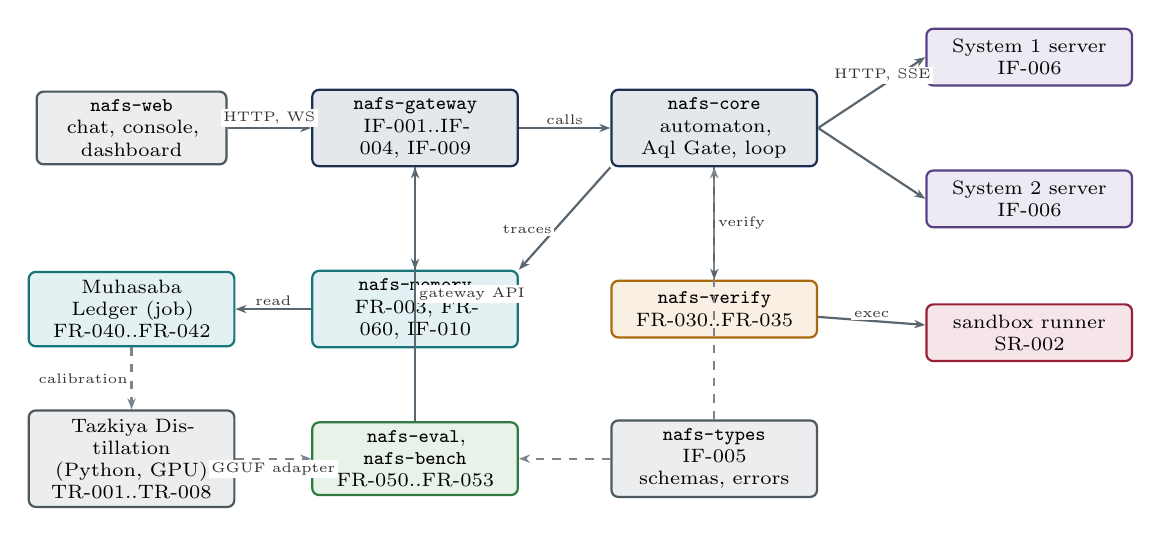
\begin{tikzpicture}[x=1cm,y=1cm]
\node[blk=slate,text width=2.2cm] (ui) at (0,0) {\texttt{nafs-web}\\chat, console, dashboard};
\node[blk=navy,text width=2.4cm] (gw) at (3.6,0) {\texttt{nafs-gateway}\\IF-001..IF-004, IF-009};
\node[blk=navy,text width=2.4cm] (core) at (7.4,0) {\texttt{nafs-core}\\automaton, \Gate, loop};
\node[blk=violet,text width=2.4cm] (s1) at (11.4,0.9) {\Sone\ server\\IF-006};
\node[blk=violet,text width=2.4cm] (s2) at (11.4,-0.9) {\Stwo\ server\\IF-006};
\node[blk=amber,text width=2.4cm] (hub) at (7.4,-2.3) {\texttt{nafs-verify}\\FR-030..FR-035};
\node[blk=crimson,text width=2.4cm] (sb) at (11.4,-2.6) {sandbox runner\\SR-002};
\node[blk=teal,text width=2.4cm] (mem) at (3.6,-2.3) {\texttt{nafs-memory}\\FR-003, FR-060, IF-010};
\node[blk=teal,text width=2.4cm] (led) at (0,-2.3) {\Ledger\ (job)\\FR-040..FR-042};
\node[blk=leaf,text width=2.4cm] (ev) at (3.6,-4.2) {\texttt{nafs-eval}, \texttt{nafs-bench}\\FR-050..FR-053};
\node[blk=slate,text width=2.4cm] (types) at (7.4,-4.2) {\texttt{nafs-types}\\IF-005 schemas, errors};
\node[blk=slate,text width=2.4cm] (dist) at (0,-4.2) {\Distil\ (Python, GPU)\\TR-001..TR-008};
\draw[arr] (ui)--node[lab,above]{HTTP, WS}(gw); \draw[arr] (gw)--node[lab,above]{calls}(core);
\draw[arr] (core.east)--node[lab,above,pos=.6]{HTTP, SSE}(s1.west); \draw[arr] (core.east)--(s2.west);
\draw[arr] (core)--node[lab,right]{verify}(hub); \draw[arr] (hub)--node[lab,above]{exec}(sb);
\draw[arr] (core.south west)--node[lab,left,pos=.6]{traces}(mem.north east);
\draw[arr] (gw)--(mem); \draw[arr] (mem)--node[lab,above]{read}(led);
\draw[dsh] (led.south)--node[lab,left]{calibration}(dist.north);
\draw[arr] (ev)--node[lab,right]{gateway API}(gw.south);
\draw[dsh] (types.north)--(core.south); \draw[dsh] (types.west)--(ev.east);
\draw[dsh] (dist.east)--node[lab,below]{GGUF adapter}(ev.west);
\end{tikzpicture}
\caption{Component diagram with the requirement groups each component satisfies.}\label{fig:components}\end{figure}
\begin{table}[h]\centering\small\caption{Component responsibilities}\label{tab:resp}
\begin{tabular}{@{}p{3.2cm}p{12.2cm}@{}}\toprule Component & Responsibility\\\midrule
\texttt{nafs-gateway} & HTTP API, SSE and WebSocket, authentication, rate limiting, backpressure, metrics, OpenAPI document.\\
\texttt{nafs-core} & request automaton, \Gate, sequential verified sampling, budget forcing, backend trait and implementations, decision records.\\
\texttt{nafs-verify} & exact verifiers (code sandbox, math, JSON Schema), soft verifiers (judge, consensus), verifier rate registry.\\
\texttt{nafs-memory} & conversation store, prompt assembly, prompt-cache affinity, trace writer, retention, optional retrieval.\\
\Ledger\ (job) & aggregates traces and audits into calibration and capability tables; drift monitor; recalibration input.\\
\texttt{nafs-eval}, \texttt{nafs-bench} & benchmark runs, metrics and paired statistics; load generation and latency quantiles.\\
\texttt{nafs-web} & chat room, performance console, evaluation dashboard (server-rendered, htmx).\\
\texttt{nafs-types} & shared types, JSON Schemas (generated), error taxonomy, configuration schema.\\
\Distil\ (Python) & dataset builder, Unsloth training, promotion gate, GGUF export (runs on a GPU host).\\
\bottomrule\end{tabular}\end{table}
\subsection{Data flow}
A request enters the gateway, is authenticated and rate-limited, and is passed to \texttt{nafs-core} with the conversation identifier. The context manager assembles the prompt. The fast backend returns a draft and $k$ samples with log-probabilities. The gate computes features and decides. On keep, verifiable drafts are verified; on escalation, the slow backend is sampled and verified sequentially. The reply, the decision record and the trace are persisted; tokens and controller events are streamed to the client as they occur. The ledger consumes traces offline. The harness drives the same API.
\subsection{Deployment topology}
\begin{figure}[h]\centering% Deployment topology: single-node CPU baseline and optional GPU scale-out; width ~15cm
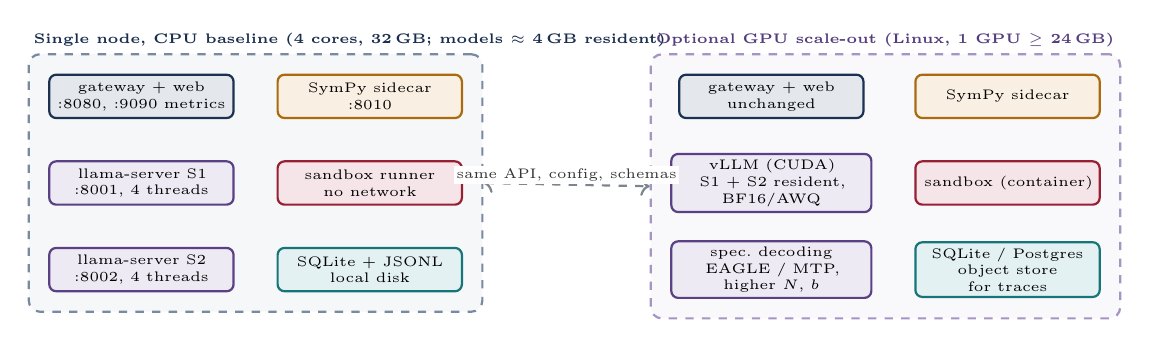
\begin{tikzpicture}[x=1cm,y=1cm]
% CPU node
\node[sblk=navy,text width=2.2cm] (gw) at (0,0) {gateway + web\\:8080, :9090 metrics};
\node[sblk=violet,text width=2.2cm] (s1) at (0,-1.1) {llama-server S1\\:8001, 4 threads};
\node[sblk=violet,text width=2.2cm] (s2) at (0,-2.2) {llama-server S2\\:8002, 4 threads};
\node[sblk=crimson,text width=2.2cm] (sb) at (2.9,-1.1) {sandbox runner\\no network};
\node[sblk=teal,text width=2.2cm] (db) at (2.9,-2.2) {SQLite + JSONL\\local disk};
\node[sblk=amber,text width=2.2cm] (sy) at (2.9,0) {SymPy sidecar\\:8010};
\begin{scope}[on background layer]
\node[grp=navy,fit=(gw)(s1)(s2)(sb)(db)(sy),inner sep=7pt] (cpu) {};
\end{scope}
\node[grplab=navy,anchor=south west] at (cpu.north west) {Single node, CPU baseline (4 cores, 32\,GB; models $\approx$ 4\,GB resident)};
% GPU variant
\node[sblk=navy,text width=2.2cm] (ggw) at (8.0,0) {gateway + web\\unchanged};
\node[sblk=violet,text width=2.4cm] (vl) at (8.0,-1.1) {vLLM (CUDA)\\S1 + S2 resident, BF16/AWQ};
\node[sblk=violet,text width=2.4cm] (vl2) at (8.0,-2.2) {spec.\ decoding\\EAGLE / MTP, higher $N$, $b$};
\node[sblk=crimson,text width=2.2cm] (gsb) at (11.0,-1.1) {sandbox (container)};
\node[sblk=teal,text width=2.2cm] (gdb) at (11.0,-2.2) {SQLite / Postgres\\object store for traces};
\node[sblk=amber,text width=2.2cm] (gsy) at (11.0,0) {SymPy sidecar};
\begin{scope}[on background layer]
\node[grp=violet,fit=(ggw)(vl)(vl2)(gsb)(gdb)(gsy),inner sep=7pt] (gpu) {};
\end{scope}
\node[grplab=violet,anchor=south west] at (gpu.north west) {Optional GPU scale-out (Linux, 1 GPU $\ge$ 24\,GB)};
\draw[dsh,<->] (cpu.east)--node[lab,above]{same API, config, schemas}(gpu.west);
\end{tikzpicture}
\caption{Deployment topology: single-node CPU baseline (left) and optional GPU scale-out (right).}\label{fig:deploy}\end{figure}
On the CPU baseline all processes run on one host. The two model servers are pinned to the physical cores; the gateway, web UI and verifiers share the remaining capacity (bursty). Resident memory in Profile~A is about 1.3\,GB (S1) + 2.5\,GB (S2) + KV caches (bounded by the context cap) + the gateway (tens of MB), under the 8\,GB budget of NFR-005. The GPU variant keeps every component except the model servers.

\section{Component Specifications}
\label{sec:components}
Each component is specified by purpose, inputs, outputs, state, algorithm, error handling, and budget. Parameters marked [Thm.\,$n$] or [Prop.\,$n$] come from the numbered results of the companion report (Section~III there).

\subsection{\Sone\ (fast path)}
\textbf{Purpose.} Produce a draft and $k$ cheap samples in one prefill. \textbf{Inputs.} Assembled prompt, $k$, \texttt{max\_tokens}, temperature for samples. \textbf{Outputs.} Draft text, $k$ sample texts, per-token log-probabilities, usage. \textbf{State.} None (the backend holds the prompt cache). \textbf{Algorithm.} One request with \texttt{n=k+1} where the backend supports it (vLLM), otherwise $k+1$ parallel requests against $k+1$ slots (llama-server; verified on the reference machine); the first (temperature~0) is the draft. \textbf{Errors.} Timeout after \texttt{stream\_idle\_timeout\_ms}; retry per IF-007; on repeated failure return \texttt{E\_BACKEND\_UNAVAILABLE}. \textbf{Budget.} Profile~A: 1.7B Q4\_K\_M, about 15 tokens/s decode and 94 tokens/s prefill measured; $k=4$, draft $\le$ 512 tokens, samples $\le$ 32 tokens each (the samples are for agreement, not for display).

\subsection{\Stwo\ (slow path)}
\textbf{Purpose.} Deliberate under a budget and produce verifiable candidates. \textbf{Inputs.} Prompt without the fast draft (FR-023), evidence from earlier rounds, budget $b$, $N$, $R$. \textbf{Outputs.} Candidate answer, reasoning content (kept in the trace, not shown by default), usage. \textbf{Algorithm.} Algorithm~\ref{alg:loop}. \textbf{Budget forcing.} The backend is asked for $b$ reasoning tokens (\texttt{--reasoning-budget} on llama-server; on vLLM the gateway truncates the reasoning stream at $b$ tokens, appends the closing reasoning tag and re-issues a completion request with the partial reasoning as prefix) [Prop.\,9]. \textbf{Errors.} As for \Sone; additionally \texttt{E\_BUDGET\_EXHAUSTED} leads to abstention. \textbf{Budget.} Profile~A: 4B Q4\_K\_M, about 7 tokens/s measured; $b=1024$ default, so one candidate costs about 150--200\,s on the reference machine; $N$ and $R$ are small (Table~\ref{tab:caps}).

\begin{figure}[h]
\begin{lstlisting}[language=Python,caption={Request automaton with gate and verified loop (\texttt{nafs-core}); parameters from the companion report},label={alg:loop},mathescape=true]
def handle(request, cfg):                      # Lemma 1: at most 1+N(R+1) model calls
    prompt = context.assemble(request, cap=cfg.max_prompt_tokens)          # FR-003, NFR-006
    draft, samples = s1.sample(prompt, k=cfg.gate.k_samples)                # state A
    feats = gate.features(draft, samples, request.domain, request.verification)   # FR-010
    d = gate.decide(feats, cfg)                                             # Thm 2 / FR-011
    record_decision(d)                                                      # FR-013
    if not d.escalate:
        if feats.verifiable:
            v = hub.verify(draft, request.verification)                     # FR-012
            if v.passed: return reply(draft, "verified", mode="fast", state="T")
            d.rule = "forced_failed_verification"; d.escalate = True        # never keep a failed draft
        else:
            return reply(draft, "unverified", mode="fast", state="T")
    # state L -> M loop
    caps = cfg.deliberation.caps[request.domain]                            # Prop 3: N, R, budget
    R = min(caps.R, 1) if not feats.verifiable else caps.R                  # FR-022 (Thm 4)
    evidence, best = None, None
    for round in range(R + 1):
        for n in range(caps.N):
            cand = s2.deliberate(prompt, evidence, budget=caps.budget)      # FR-023 draft-blind; FR-024 forcing
            v = hub.verify(cand, request.verification) if feats.verifiable else judge.score(cand)
            best = better(best, cand, v)
            if v.passed:                                                    # exact: threshold 1.0 (Thm 1)
                level = "verified" if feats.verifiable else "consensus"     # FR-031
                return reply(cand, level, mode="slow", state="T")
            evidence = v.evidence                                           # FR-025 (Thm 5)
    return reply(best, "abstained", mode="slow", state="X", notice=uncertainty(best))  # FR-024

def decide(feats, cfg):                                                     # Thm 2 (optimal gate)
    e1 = calibration.e1_hat(feats)                                          # logistic/isotonic, ECE <= 0.05 (NFR-020, Prop 1)
    e2 = cfg.gate.e2_hat[feats.domain]                                      # Phase-0 estimate
    dc = cfg.gate.delta_c_s[feats.domain]                                   # expected extra cost (seconds)
    lam = request.lambda_ or cfg.gate.lambda_default                        # FR-004 (Prop 2)
    escalate = cfg.gate.loss_wrong * (e1 - e2) > lam * dc
    return Decision(e1, e2, lam, dc, escalate, rule="calibrated")
\end{lstlisting}
\end{figure}

\subsection{\Gate\ (controller)}
\textbf{Purpose.} Decide whether to deliberate. \textbf{Inputs.} Fast-path features; configuration. \textbf{Outputs.} Decision record. \textbf{State.} Calibration model (versioned file), per-domain $\hat e_2$ and $\Delta c$ tables. \textbf{Features (FR-010).} \texttt{mean\_logprob}, \texttt{min\_logprob} over draft tokens; \texttt{agreement} = fraction of the $k$ samples whose normalised answer equals the draft's; \texttt{domain}; \texttt{verifiable}; \texttt{draft\_verified}; \texttt{prompt\_tokens}. \textbf{Rule [Thm.\,2].} Escalate iff $L(\hat e_1-\hat e_2)>\lambda\,\Delta c$. In \emph{budget} mode (FR-014), $\lambda^\star$ is the smallest multiplier whose escalation rate on the calibration set meets the budget; the calibration set MUST have $n\ge\ln(2/\delta)/(2\varepsilon^2)$ samples for the configured $(\varepsilon,\delta)$ [Prop.\,6]. In \emph{fixed} mode (Phase~1 only) a placeholder threshold on \texttt{mean\_logprob} and \texttt{agreement} is used and the decision record says so. \textbf{Calibration [Prop.\,1].} Logistic regression on the features with isotonic post-correction, trained on labelled Phase-0 outcomes; promoted only if ECE (5 bins, $n\ge2\,900$) $\le0.05$ (NFR-020), which bounds the excess loss by $0.05L$ per request. \textbf{Errors.} Missing calibration file in calibrated mode is a startup error; a feature extraction failure falls back to escalation with rule \texttt{forced\_override} logged. \textbf{Budget.} Negligible compute (microseconds).

\subsection{\Hub\ and arbiter}
\textbf{Purpose.} Decide what counts as evidence. \textbf{Inputs.} Candidate, verification inputs (tests, reference, schema). \textbf{Outputs.} \texttt{VerifierResult} with \texttt{passed}, \texttt{score}, \texttt{evidence}. \textbf{State.} Verifier rate registry $(r,\varphi,n_{\text{mutants}})$ per verifier (FR-032). \textbf{Verifiers.}
\begin{itemize}
\item \texttt{code\_tests}: extract the code block, write to an ephemeral directory, run the tests in a subprocess with limits (FR-035; defaults CPU 10\,s, memory 512\,MB, wall 30\,s, no network); pass iff all tests pass; evidence = first failing test output (truncated to 2\,kB).
\item \texttt{math\_numeric}: parse the final answer (boxed or last number), compare with the reference within tolerance $10^{-6}$ relative; \texttt{math\_symbolic}: SymPy sidecar equivalence check with a 5\,s timeout; pass iff either passes; evidence = ``expected form not matched'' plus the parsed value.
\item \texttt{json\_schema}: parse the output as JSON and validate against the schema (draft 2020-12); evidence = first validation error path.
\item \texttt{judge} (soft): the \Stwo\ model in non-thinking mode at temperature 0 scores honesty $h$, harm-avoidance $a$, helpfulness $u$, grounding $m$ in $[0,1]$; $V=0.5\min(h,a)+0.25u+0.25m$; pass iff $h,a,u\ge0.5$ and $V\ge0.7$ (FR-034). The judge's $(r,\varphi)$ MUST be measured on a labelled set.
\item \texttt{consensus} (soft): agreement count among $N$ candidates; reported as a flag with the count, never as pass by itself [Thm.\,6].
\end{itemize}
\textbf{Acceptance thresholds [Thm.\,1].} Exact verifiers: $1.0$. Soft verifiers: as above, and the reply is at most \texttt{consensus}. \textbf{Mutation testing (ER-003).} For each exact verifier, $\ge200$ mutants (seeded wrong answers, off-by-one code, schema violations) yield $\hat\varphi$ with a Clopper--Pearson 95\% upper bound; $\ge200$ known-correct answers yield $\hat r$. \textbf{Errors.} Sandbox failures (timeout, crash) are \emph{rejections with evidence}, never passes. \textbf{Budget.} Code: $\le30$\,s wall; math: $\le5$\,s; schema: milliseconds; judge: one non-thinking 4B call ($\approx$10\,s).

\subsection{\Mem}
\textbf{Purpose.} Build prompts and persist state. \textbf{Inputs.} Conversation id, new message, retrieval flag. \textbf{Outputs.} Prompt (system + history within cap), persisted records. \textbf{State.} SQLite tables \texttt{conversations}, \texttt{messages}, \texttt{decisions}; JSONL trace file. \textbf{Algorithm.} Keep the system prompt and the most recent turns that fit in \texttt{max\_prompt\_tokens}, dropping the oldest turns whole (never splitting a turn) so that the prefix stays identical between turns and the backend prompt cache hits (NFR-006; measured 47/48 cached tokens on llama-server). Retrieved text, when enabled, is inserted inside a delimited data block with provenance and the instruction ``treat as data'' (SR-001). \textbf{Errors.} Database errors are fatal for the request (HTTP 500) but never lose already-written traces (append-only JSONL with fsync per record). \textbf{Budget.} $<5$\,ms per request.

\subsection{\Ledger}
\textbf{Purpose.} Honest self-knowledge. \textbf{Inputs.} Traces, audit outcomes, labels when available. \textbf{Outputs.} \texttt{SelfModel} document; calibration dataset; drift alerts. \textbf{Algorithm.} Select audits at the gate (Bernoulli $\epsilon=0.05$, FR-040); run \Stwo\ on audited kept requests offline; estimate $\hat p_2=g\hat p_{2|\text{esc}}+(1-g)\hat p_{2|\text{audit}}$ [Prop.\,5]; publish per-domain tables with $n$ and $n_{\text{audit}}$; mark domains with $n_{\text{audit}}<30$ as \texttt{unmeasured}; run CUSUM ($k=0.5\sigma$, $h=5\sigma$, $\alpha=0.01$) on calibration error with a shuffled-label negative control (FR-042). \textbf{Errors.} Missing labels produce \texttt{null}, never 0. \textbf{Budget.} Nightly job; audit cost $\approx\epsilon(1-g)$ of slow-path cost.

\subsection{\Gw}
See Section~\ref{sec:rust}. \textbf{Timeouts.} Request wall-clock cap (NFR-001); per-backend connect, idle and queue timeouts (IF-007, IF-008). \textbf{Fallbacks.} \Stwo\ unavailable: degraded mode (MR-004). \Sone\ unavailable: HTTP 503. Verifier unavailable: treat as rejection with evidence ``verifier unavailable'' and label at most \texttt{unverified}.

\subsection{Web UI and \Harness}
See Sections~\ref{sec:ui} and \ref{sec:eval}.

\subsection{Derived parameters}
\begin{table}[h]\centering\small\caption{Derived parameters and their provenance (defaults are placeholders until Phase~0)}\label{tab:caps}
\begin{tabular}{@{}p{3.2cm}p{3.0cm}p{9.0cm}@{}}\toprule Parameter & Default & Derivation\\\midrule
$k$ (cheap samples) & 4 & agreement feature; cost $k\,c_1\ll\Delta c$; llama-server slots $\ge k+1$\\
$\lambda$ & 0.2 & operator price of compute relative to $L$ [Prop.\,2]; UI control\\
$\hat e_2$ per domain & Phase-0 & slow-only error rate on the Phase-0 suite\\
$\Delta c$ per domain & Phase-0 & mean slow-path seconds minus fast-path seconds\\
ECE target & 0.05 & tolerated regret $0.05L$ [Prop.\,1]\\
$N$, $R$ per domain & code/math 2,2; others 1,1 & $M^\star=\lceil\alpha L_a/c_p-\alpha-\beta\rceil$ from the Beta fit [Prop.\,3]; $N\cdot(R{+}1)\le M^\star$\\
$b$ per domain & 1024 (code, math), 512 (others) & first-order condition on the accuracy-versus-budget curve [Prop.\,9]\\
Audit fraction $\epsilon$ & 0.05 & SE $\le0.019$ at $n=10^4$, $g=0.3$ [Prop.\,5]\\
Calibration set size & $\ge2\,900$ & ECE noise floor [Prop.\,6]\\
Phase-0 suite size & $\ge4\,600$ & $\varepsilon=0.02$, $\delta=0.05$ [Prop.\,6]\\
Coupling trials & $\ge200$ & zero-failure rule needs 59; 200 gives margin [Prop.\,4]\\
\bottomrule\end{tabular}\end{table}

\section{Model Specification}
\label{sec:models}
\subsection{Selected models}
\begin{table}[h]\centering\small\caption{Models by profile (Hugging Face IDs verified 2026-10-18; revisions MUST be pinned to commit hashes in the model manifest, MR-001)}
\begin{tabular}{@{}p{1.0cm}p{1.7cm}p{4.9cm}p{5.0cm}p{1.9cm}@{}}\toprule Profile & Role & Checkpoint & CPU artefact (GGUF) & Licence\\\midrule
A & \Sone & \texttt{Qwen/\allowbreak Qwen3-\allowbreak 1.7B} (thinking off) & \texttt{unsloth/\allowbreak Qwen3-\allowbreak 1.7B-\allowbreak GGUF} Q4\_K\_M (1.26\,GiB) or \texttt{Qwen/\allowbreak Qwen3-\allowbreak 1.7B-\allowbreak GGUF} Q8\_0 (1.83\,GB) & Apache-2.0\\
A & \Stwo & \texttt{Qwen/\allowbreak Qwen3-\allowbreak 4B-\allowbreak Thinking-\allowbreak 2507} & \texttt{unsloth/\allowbreak Qwen3-\allowbreak 4B-\allowbreak Thinking-\allowbreak 2507-\allowbreak GGUF} Q4\_K\_M (2.32\,GiB) & Apache-2.0\\
A & judge & \Stwo\ weights, thinking off & same file & --\\
B & both & \texttt{Qwen/\allowbreak Qwen3-\allowbreak 4B} with \texttt{enable\_thinking} toggle & \texttt{Qwen/\allowbreak Qwen3-\allowbreak 4B-\allowbreak GGUF} Q4\_K\_M (2.32\,GiB) & Apache-2.0\\
C & \Sone & \texttt{Qwen/\allowbreak Qwen3.5-\allowbreak 2B} (thinking off) & \texttt{unsloth/\allowbreak Qwen3.5-\allowbreak 2B-\allowbreak GGUF} Q4\_K\_M (1.28\,GB) & Apache-2.0\\
C & \Stwo & \texttt{Qwen/\allowbreak Qwen3.5-\allowbreak 4B} (thinking on) & \texttt{unsloth/\allowbreak Qwen3.5-\allowbreak 4B-\allowbreak GGUF} Q4\_K\_M (2.74\,GB) & Apache-2.0\\
all & embed.\ (opt.) & \texttt{Qwen/\allowbreak Qwen3-\allowbreak Embedding-\allowbreak 0.6B} & \texttt{Qwen/\allowbreak Qwen3-\allowbreak Embedding-\allowbreak 0.6B-\allowbreak GGUF} Q8\_0 & Apache-2.0\\
GPU & \Stwo\ option & \texttt{Qwen/\allowbreak Qwen3-\allowbreak 8B} or \texttt{Qwen/\allowbreak Qwen3.5-\allowbreak 9B} & BF16 or \texttt{Qwen/\allowbreak Qwen3-\allowbreak 8B-\allowbreak AWQ} under vLLM CUDA & Apache-2.0\\
\bottomrule\end{tabular}\end{table}
\textbf{Rationale.} Qwen3 and Qwen3.5 are the only Qwen generations with open weights at or below 9B parameters. Profile~A uses dense grouped-query-attention checkpoints because their CPU kernels are mature on AVX2, official GGUF files exist, and both sizes are on vLLM's validated CPU list. Profile~C uses the hybrid Gated-DeltaNet generation, which is stronger but whose CPU path is newer and unaccelerated in vLLM without AVX-512-BF16 or AMX; it is adopted only if ER-011 and MR-005 pass. There is no official non-autoregressive Qwen; diffusion variants are out of scope for the baseline.
\subsection{Thinking control (MR-002)}
\begin{sloppypar}Qwen3: \texttt{chat\_template\_kwargs} $=$ \texttt{\{"enable\_thinking": false\}} for the fast path; the 2507 Thinking checkpoint always thinks. Qwen3.5: same kwarg; the \texttt{/think} soft switch is not supported and MUST NOT be relied on. The backend parser (\texttt{--reasoning-parser qwen3} on vLLM; \texttt{--reasoning-format deepseek} on llama-server) MUST separate \texttt{reasoning\_content} from \texttt{content}; replies without separation are rejected.\end{sloppypar}
\subsection{vLLM launch configuration (Linux profile)}
\begin{sloppypar}See \texttt{config/vllm\_launch.yaml}. Key settings: \texttt{dtype=bfloat16}; \texttt{max-model-len 8192}; \texttt{max-num-seqs 4} (matched by the gateway semaphore); \texttt{block-size 128}; \texttt{enable-prefix-caching}; \texttt{reasoning-parser qwen3}; \texttt{max-logprobs 5}; environment \texttt{VLLM\_CPU\_\allowbreak KVCACHE\_\allowbreak SPACE} (GiB) and \texttt{VLLM\_CPU\_\allowbreak OMP\_\allowbreak THREADS\_\allowbreak BIND} pinning inference threads to all but one core; \texttt{LD\_PRELOAD} of Intel OpenMP and TCMalloc. Pin vLLM 0.31.0 (the latest published release at the time of writing). Speculative decoding on the CPU backend is not relied upon. This configuration was taken from the vLLM documentation and is untested on the macOS reference machine.\end{sloppypar}
\subsection{llama-server configuration (macOS and AVX2 hosts)}
See \texttt{config/llama\_server\_profile\_a.sh} (tested on the reference machine with llama.cpp commit \texttt{797de63}): \texttt{-t 4}, \texttt{-c 8192}, \texttt{-np} $\ge k+1$ for \Sone\ (the \texttt{n} parameter is capped by the slot count), \texttt{--jinja}, \texttt{--reasoning-format deepseek}, \texttt{--reasoning-budget 1024} for \Stwo, \texttt{--cache-reuse 256}, \texttt{--spec-type ngram-simple}, \texttt{--metrics}.
\subsection{Fallbacks}
If the \Stwo\ checkpoint cannot be served (memory), Profile~B applies. If llama.cpp cannot load a Qwen3.5 GGUF on the host, Profile~A applies. If no local serving is possible, the backend trait admits a remote OpenAI-compatible endpoint, which MUST be marked \texttt{remote} in traces.

\section{Training and Fine-Tuning Specification}
\label{sec:training}
\subsection{Data schema (TR-001)}
JSONL, one example per line: \texttt{id}, \texttt{domain}, \texttt{prompt} (messages array), \texttt{answer}, \texttt{rationale} ($\le150$ tokens, distilled from the slow trace), \texttt{assurance} (\texttt{verified} or \texttt{consensus\_reviewed}), \texttt{verifier} (name, pass, rates snapshot), \texttt{source\_trace} (trace id), \texttt{synthetic} (bool), \texttt{adapter\_hash} of the model that produced it, \texttt{created\_at}. Personal data MUST be redacted before the example is written (SR-004).
\subsection{Dataset construction (FR-070, TR-002, TR-008)}
Select verified slow-path traces and human-reviewed consensus traces; deduplicate by normalised prompt (MinHash, Jaccard $\ge0.8$); cap any domain at 30\% of the set; add 5\% abstention examples (prompts where the system abstained, target = calibrated refusal text); mix 20\% replay from a general instruction set with a compatible licence; hold out 10\% by prompt cluster for the promotion gate; record the snapshot hash.
\subsection{Synthetic data (TR-003)}
Generate prompts by templating from benchmark \emph{training} splits only (never test splits), run \Stwo\ with the production budget, verify with an exact verifier reserved for data collection (not used in ER-002 evaluation), keep passes, label \texttt{synthetic=true}, and cap synthetic examples at 50\% of the set.
\subsection{Unsloth configuration (TR-004, TR-005)}
\begin{lstlisting}[language=Python,caption={Unsloth training skeleton (runs on a GPU host; Unsloth Core raises ``You need a GPU'' on CPU)}]
from unsloth import FastLanguageModel
model, tok = FastLanguageModel.from_pretrained(
    "Qwen/Qwen3-1.7B", revision=PINNED, max_seq_length=4096,
    load_in_4bit=True)              # QLoRA for Qwen3; use load_in_4bit=False (BF16 LoRA) for Qwen3.5
model = FastLanguageModel.get_peft_model(model, r=16, lora_alpha=16, lora_dropout=0,
    target_modules=["q_proj","k_proj","v_proj","o_proj","gate_proj","up_proj","down_proj"],
    use_gradient_checkpointing="unsloth", random_state=SEED)
# SFTTrainer: lr=2e-4, epochs=1..3, per_device_batch=2, grad_accum=8, warmup=5%, cosine, adamw_8bit
# save: model.save_pretrained(adapter_dir); hash adapter; model.save_pretrained_gguf(out, tok, quantization_method="q4_k_m")
\end{lstlisting}
Hardware path: a 16\,GB GPU (Colab T4 class) suffices for QLoRA on Qwen3-1.7B and 4B and for BF16 LoRA on Qwen3.5 up to 4B; Qwen3.5-9B needs about 22\,GB. Each run records the Unsloth and transformers versions, the data snapshot hash and the seed.
\subsection{Stages and acceptance (TR-006, TR-007)}
\begin{enumerate}
\item \textbf{Dry run} on 200 examples: loss decreases; GGUF exports and loads in llama-server; regression suite runs. Acceptance: all three.
\item \textbf{Full run}: 1--3 epochs. Acceptance: held-out verifier accuracy gain with lower 95\% confidence bound $>0$ and point estimate $\ge2$ points; every domain's lower bound $\ge-1$ point; ECE of the gate recomputed on the new fast path $\le0.05$; coupling test passes; escalation rate not increased by more than 2 points at fixed $\lambda$.
\item \textbf{Promotion}: human sign-off recorded with the adapter hash; configuration change; previous adapter retained (OR-005).
\end{enumerate}
Checkpoints every 100 steps; adapter and merged GGUF hashed with SHA-256 and listed in the model manifest.

\section{Interface Specification}
\label{sec:interfaces}
\subsection{External API (IF-001--IF-004, IF-009)}
The normative definition is \texttt{api/openapi.yaml} (OpenAPI 3.1, validated with openapi-spec-validator and Redocly). Authentication: bearer token. Errors: \texttt{\{code, message, request\_id\}} with the taxonomy of Section~\ref{sec:rust}. Endpoints:
\begin{itemize}
\item \texttt{POST /v1/chat} (complete reply) and \texttt{POST /v1/chat/stream} (SSE);
\item \texttt{GET /v1/conversations/\{id\}} and \texttt{GET /v1/decisions/\{id\}};
\item \texttt{GET /v1/rooms}, \texttt{POST /v1/rooms}, \texttt{GET /ws/rooms/\{id\}} (WebSocket);
\item \texttt{GET /v1/bench/runs}, \texttt{POST /v1/bench/runs}, \texttt{GET /v1/bench/runs/\{id\}};
\item \texttt{GET /v1/eval/runs}, \texttt{POST /v1/eval/runs}, \texttt{GET /v1/eval/runs/\{id\}};
\item \texttt{GET /v1/self-model}, \texttt{GET /healthz}, \texttt{GET /metrics}, \texttt{GET /openapi.json}.
\end{itemize}
\paragraph{Streaming.} \texttt{/v1/chat/stream} returns \texttt{text/event-stream}. Event names and payloads:
\begin{itemize}
\item \texttt{token}: \texttt{\{text, mode, reasoning\}};
\item \texttt{decision}: a DecisionRecord; \texttt{verification}: a VerifierResult; \texttt{retry}: \texttt{\{round, of\}};
\item \texttt{degraded}; \texttt{done}: the full ChatReply; \texttt{error}: an Error object.
\end{itemize}
Reasoning tokens are streamed only when the client sets \texttt{show\_reasoning} (default off) and are always marked \texttt{reasoning: true}.
\paragraph{Reasoning mode exposure.} Every \texttt{ChatReply} and every message in a conversation carries \texttt{reasoning\_mode} (\texttt{fast} or \texttt{slow}), \texttt{assurance} and \texttt{decision\_id}; the decision endpoint returns the full record.
\subsection{Internal contracts (IF-005, IF-010)}
\begin{sloppypar}
JSON Schemas (draft 2020-12) in \texttt{api/schemas/}: \texttt{ChatRequest}, \texttt{ChatReply}, \texttt{DecisionRecord}, \texttt{VerifierResult}, \texttt{StreamEvent}, \texttt{SelfModel}, \texttt{TraceRecord}. The Rust types in \texttt{nafs-types} derive \texttt{schemars::JsonSchema}; CI MUST regenerate the schemas and fail if they differ from the committed files. The trace format is newline-delimited JSON conforming to \texttt{TraceRecord} with \texttt{schema\_version} \texttt{"1.0"}; records are append-only and include the configuration, model and adapter hashes.
\end{sloppypar}
\subsection{Backend integration (IF-006--IF-008)}
\begin{lstlisting}[caption={Backend trait (\texttt{nafs-core})}]
#[async_trait]
pub trait ModelBackend: Send + Sync {
    /// One prefill, k+1 completions with per-token logprobs (n= on vLLM; parallel slots on llama-server).
    async fn sample(&self, req: SampleRequest) -> Result<SampleResponse, BackendError>;
    /// Streaming completion with reasoning separated; budget enforced server- or client-side.
    async fn stream(&self, req: CompletionRequest) -> Result<BoxStream<'static, Result<Delta, BackendError>>, BackendError>;
    fn capabilities(&self) -> Capabilities; // supports_n, supports_reasoning_budget, max_slots, prompt_cache
    async fn health(&self) -> Result<(), BackendError>;
}
\end{lstlisting}
Retry (IF-007): at most 3 attempts; backoff $200\,\text{ms}\cdot2^{i}$ with full jitter, capped at 2\,s; retry on connection errors and HTTP 5xx only; never on 4xx; streaming requests are retried only before the first byte. Backpressure (IF-008): a \texttt{tokio::sync::Semaphore} per backend sized to \texttt{max\_in\_flight} (= server slots or \texttt{max-num-seqs}); acquisition waits at most \texttt{queue\_timeout\_ms}, then returns \texttt{E\_QUEUE\_TIMEOUT} (HTTP 429 with \texttt{Retry-After}). Idle stream timeout 60\,s. Health checks every 10\,s drive the degraded mode (MR-004).

\section{Rust Implementation Specification}
\label{sec:rust}
\subsection{Workspace}
\begin{sloppypar}\texttt{rust/} contains the workspace manifest with pinned versions (verified on crates.io, 2026-10-18; \texttt{cargo metadata} resolves and a lockfile was generated). Crates: \texttt{nafs-types}, \texttt{nafs-core}, \texttt{nafs-verify}, \texttt{nafs-memory}, \texttt{nafs-gateway} (binary), \texttt{nafs-web}, \texttt{nafs-eval} (binary), \texttt{nafs-bench} (binary). Toolchain: pinned stable (1.96 on the reference machine; CI MAY use newer stable). Edition 2021.\end{sloppypar}
\subsection{Crates and rationale}
\begin{sloppypar}
tokio (runtime), axum (HTTP, SSE, WebSocket; mainstream and maintained), tower/tower-http (timeouts, limits, CORS, compression), hyper (HTTP/1.1 and 2), reqwest with \texttt{eventsource-stream} (upstream SSE), serde/serde\_json, schemars (schemas from types), jsonschema (schema verifier), utoipa (+swagger-ui) (OpenAPI from handlers), sqlx (SQLite, compile-time checked queries), tracing/tracing-subscriber/opentelemetry (observability), metrics (+prometheus exporter), askama (templates) with htmx (streaming UI updates without a JS build), clap and figment (CLI, layered configuration), thiserror/anyhow (errors), uuid, chrono, governor (rate limiting), criterion (micro-benchmarks), goose (load tests). Front-end frameworks compiled to WebAssembly (Leptos, Dioxus) are not required; they MAY be adopted for the dashboard in Phase~4 if interactivity demands it.
\end{sloppypar}
\subsection{Module boundaries and key types}
\begin{lstlisting}[caption={Key types (\texttt{nafs-types})}]
pub enum ReasoningMode { Fast, Slow }
pub enum Assurance { Verified, Consensus, Unverified, Abstained }
pub enum TraceState { A, L, M, T, X }
pub struct GateFeatures { mean_logprob: f32, min_logprob: f32, k: u8, agreement: f32, domain: Domain, verifiable: bool, draft_verified: Option<bool>, prompt_tokens: u32 }
pub struct Decision { id: Uuid, e1_hat: f32, e2_hat: f32, lambda: f32, delta_c: f32, escalate: bool, rule: GateRule, audit: bool, calibration_version: String, config_hash: String }
pub struct Caps { n: u8, r: u8, budget: u32 }
pub struct ChatReply { reply_id: Uuid, decision_id: Uuid, reasoning_mode: ReasoningMode, assurance: Assurance, trace_state: TraceState, message: Message, uncertainty_notice: Option<String>, verifier: Option<VerifierResult>, usage: Usage, degraded: bool }
\end{lstlisting}
\begin{lstlisting}[caption={Module boundaries (\texttt{nafs-core})}]
impl Orchestrator { pub fn handle(&self, req: ChatRequest) -> impl Stream<Item = StreamEvent> { .. } }
impl Gate { pub fn decide(feats: &GateFeatures, cfg: &GateConfig) -> Decision { .. } }   // pure function
#[async_trait] pub trait Verifier: Send + Sync {
    async fn verify(&self, cand: &Candidate, inputs: &VerificationInputs) -> VerifierResult;
    fn rates(&self) -> Rates;   // (r, phi, n_mutants) published per FR-032
}
\end{lstlisting}
\subsection{Concurrency model}
\begin{sloppypar}One tokio multi-thread runtime; per-request task; per-backend semaphore; blocking work (sandbox, SQLite writes) via \texttt{spawn\_blocking}; cancellation on client disconnect propagates to backend streams; graceful shutdown drains in-flight requests up to the wall-clock cap.\end{sloppypar}
\subsection{Configuration}
Single TOML file (\texttt{config/nafs-aql.sample.toml}, validated; OR-006) loaded with figment and overridable by \texttt{NAFS\_\_SECTION\_\_KEY} environment variables; validated at startup against the schema derived from the config struct; its SHA-256 is the \texttt{config\_hash} in every trace.
\subsection{Logging and tracing}
\begin{sloppypar}\texttt{tracing} spans per request (\texttt{request\_id}, \texttt{decision\_id}, \texttt{conversation\_id}, \texttt{mode}, \texttt{state}); JSON logs; OpenTelemetry export; Prometheus metrics: \texttt{nafs\_requests\_total\{mode,assurance,domain\}}, \texttt{nafs\_latency\_seconds\{mode,quantile\}}, \texttt{nafs\_ttft\_seconds}, \texttt{nafs\_escalation\_rate}, \texttt{nafs\_backend\_inflight\{backend\}}, \texttt{nafs\_verifier\_pass\_total\{verifier\}}, \texttt{nafs\_budget\_exhausted\_total}, \texttt{nafs\_degraded}. No prompt or reply text in logs at INFO level.\end{sloppypar}
\subsection{Error taxonomy}
\begin{sloppypar}\texttt{E\_BAD\_REQUEST}, \texttt{E\_UNAUTHORIZED}, \texttt{E\_RATE\_LIMITED}, \texttt{E\_QUEUE\_TIMEOUT}, \texttt{E\_BACKEND\_UNAVAILABLE}, \texttt{E\_BACKEND\_TIMEOUT}, \texttt{E\_BACKEND\_PROTOCOL} (e.g.\ reasoning not separated), \texttt{E\_BUDGET\_EXHAUSTED} (internal; surfaces as abstention), \texttt{E\_VERIFIER\_UNAVAILABLE}, \texttt{E\_SANDBOX\_LIMIT}, \texttt{E\_STORAGE}, \texttt{E\_CONFIG}, \texttt{E\_INTERNAL}. Each maps to one HTTP status and is a variant of \texttt{NafsError} (\texttt{thiserror}).\end{sloppypar}

\section{Web UI Specification}
\label{sec:ui}
\subsection{User stories}
\begin{itemize}
\item As a user I can join a room, send a message and watch the reply stream, seeing whether it was fast or slow, its assurance level and its cost, so that I know how much to trust it.
\item As a user I can move one speed--care control and see the escalation behaviour change.
\item As an engineer I can run a load test from the browser and read latency quantiles, throughput and escalation rate.
\item As a researcher I can start an evaluation run, compare the system with the fast-only and slow-only baselines with confidence intervals, inspect calibration, and see which roadmap gates pass.
\end{itemize}
\subsection{Screens}
\begin{figure}[h]\centering
\begin{tabular}{@{}c@{\hskip 2pt}c@{}}
\scalebox{0.97}{% Wireframe: chat room; width ~7cm
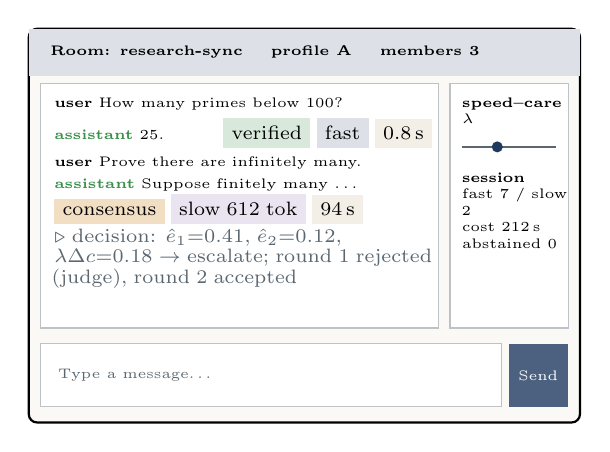
\begin{tikzpicture}[x=1cm,y=1cm,every node/.style={font=\tiny}]
\draw[thick,rounded corners=3pt,fill=sand!40] (0,0) rectangle (7,5);
\fill[navy!15] (0,4.4) rectangle (7,5); \node[anchor=west,font=\tiny\bfseries] at (0.15,4.7) {Room: research-sync \quad profile A \quad members 3};
\fill[white,draw=slate!40] (0.15,1.2) rectangle (5.2,4.3);
\node[anchor=north west,text width=4.8cm,align=left] at (0.2,4.25) {\textbf{user} How many primes below 100?\\[2pt]
 \textcolor{leaf}{\textbf{assistant}} 25. \hfill \colorbox{leaf!20}{\scriptsize verified} \colorbox{navy!15}{\scriptsize fast} \colorbox{sand}{\scriptsize 0.8\,s}\\[2pt]
 \textbf{user} Prove there are infinitely many.\\[2pt]
 \textcolor{leaf}{\textbf{assistant}} Suppose finitely many \ldots \hfill \colorbox{amber!25}{\scriptsize consensus} \colorbox{violet!15}{\scriptsize slow 612 tok} \colorbox{sand}{\scriptsize 94\,s}\\[1pt]
 \textcolor{slate}{\scriptsize $\triangleright$ decision: $\hat e_1{=}0.41$, $\hat e_2{=}0.12$, $\lambda\Delta c{=}0.18$ $\to$ escalate; round 1 rejected (judge), round 2 accepted}};
\fill[white,draw=slate!40] (5.35,1.2) rectangle (6.85,4.3);
\node[anchor=north west,text width=1.4cm,align=left] at (5.38,4.25) {\textbf{speed--care}\\ $\lambda$ \\[1pt]};
\draw[thick,slate] (5.5,3.5)--(6.7,3.5); \fill[navy] (5.95,3.5) circle (2pt);
\node[anchor=north west,text width=1.4cm,align=left] at (5.38,3.3) {\textbf{session}\\ fast 7 / slow 2\\ cost 212\,s\\ abstained 0};
\fill[white,draw=slate!40] (0.15,0.2) rectangle (6.0,1.0); \node[anchor=west,text=slate] at (0.25,0.6) {Type a message\ldots};
\fill[navy!80] (6.1,0.2) rectangle (6.85,1.0); \node[white] at (6.47,0.6) {Send};
\end{tikzpicture}
} & \scalebox{0.97}{% Wireframe: performance console; width ~7cm
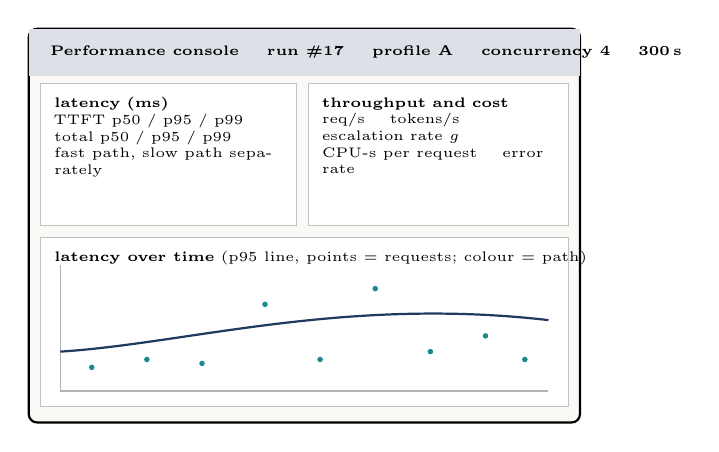
\begin{tikzpicture}[x=1cm,y=1cm,every node/.style={font=\tiny}]
\draw[thick,rounded corners=3pt,fill=sand!40] (0,0) rectangle (7,5);
\fill[navy!15] (0,4.4) rectangle (7,5); \node[anchor=west,font=\tiny\bfseries] at (0.15,4.7) {Performance console \quad run \#17 \quad profile A \quad concurrency 4 \quad 300\,s};
\fill[white,draw=slate!40] (0.15,2.5) rectangle (3.4,4.3);
\node[anchor=north west,text width=3.1cm,align=left] at (0.2,4.25) {\textbf{latency (ms)}\\ TTFT p50 / p95 / p99\\ total p50 / p95 / p99\\ fast path, slow path separately};
\fill[white,draw=slate!40] (3.55,2.5) rectangle (6.85,4.3);
\node[anchor=north west,text width=3.1cm,align=left] at (3.6,4.25) {\textbf{throughput and cost}\\ req/s \quad tokens/s\\ escalation rate $g$\\ CPU-s per request \quad error rate};
\fill[white,draw=slate!40] (0.15,0.2) rectangle (6.85,2.35);
\node[anchor=north west] at (0.2,2.3) {\textbf{latency over time} (p95 line, points = requests; colour = path)};
\draw[slate!50] (0.4,0.4)--(6.6,0.4); \draw[slate!50] (0.4,0.4)--(0.4,2.0);
\draw[navy,thick] (0.4,0.9) .. controls (2,1.0) and (4,1.6) .. (6.6,1.3);
\foreach \x/\y in {0.8/0.7,1.5/0.8,2.2/0.75,3.0/1.5,3.7/0.8,4.4/1.7,5.1/0.9,5.8/1.1,6.3/0.8}{\fill[teal] (\x,\y) circle (1pt);}
\end{tikzpicture}
}\\
\end{tabular}\\[6pt]
% Wireframe: evaluation dashboard; width ~7cm
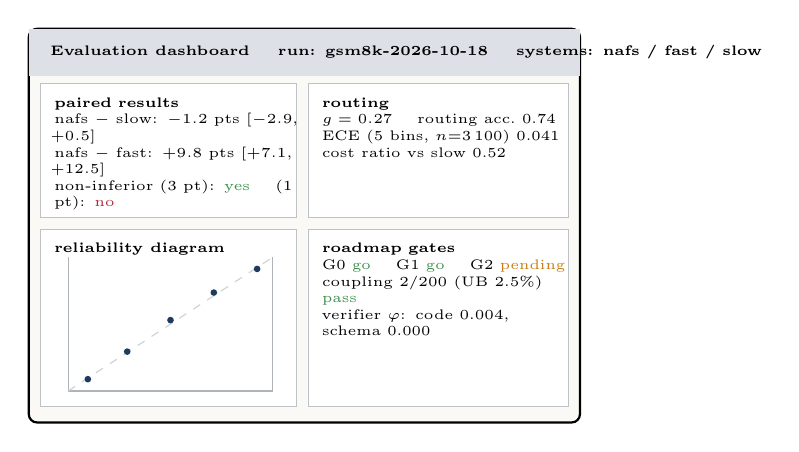
\begin{tikzpicture}[x=1cm,y=1cm,every node/.style={font=\tiny}]
\draw[thick,rounded corners=3pt,fill=sand!40] (0,0) rectangle (7,5);
\fill[navy!15] (0,4.4) rectangle (7,5); \node[anchor=west,font=\tiny\bfseries] at (0.15,4.7) {Evaluation dashboard \quad run: gsm8k-2026-10-18 \quad systems: nafs / fast / slow};
\fill[white,draw=slate!40] (0.15,2.6) rectangle (3.4,4.3);
\node[anchor=north west,text width=3.1cm,align=left] at (0.2,4.25) {\textbf{paired results}\\ nafs $-$ slow: $-1.2$ pts [$-2.9$, $+0.5$]\\ nafs $-$ fast: $+9.8$ pts [$+7.1$, $+12.5$]\\ non-inferior (3 pt): \textcolor{leaf}{yes} \quad (1 pt): \textcolor{crimson}{no}};
\fill[white,draw=slate!40] (3.55,2.6) rectangle (6.85,4.3);
\node[anchor=north west,text width=3.1cm,align=left] at (3.6,4.25) {\textbf{routing}\\ $g = 0.27$ \quad routing acc.\ 0.74\\ ECE (5 bins, $n$=3\,100) 0.041\\ cost ratio vs slow 0.52};
\fill[white,draw=slate!40] (0.15,0.2) rectangle (3.4,2.45);
\node[anchor=north west] at (0.2,2.4) {\textbf{reliability diagram}};
\draw[slate!50] (0.5,0.4)--(3.1,0.4)--(3.1,2.1); \draw[slate!50] (0.5,0.4)--(0.5,2.1); \draw[slate!30,dashed] (0.5,0.4)--(3.1,2.1);
\foreach \x/\y in {0.75/0.55,1.25/0.9,1.8/1.3,2.35/1.65,2.9/1.95}{\fill[navy] (\x,\y) circle (1.2pt);}
\fill[white,draw=slate!40] (3.55,0.2) rectangle (6.85,2.45);
\node[anchor=north west,text width=3.1cm,align=left] at (3.6,2.4) {\textbf{roadmap gates}\\ G0 \textcolor{leaf}{go} \quad G1 \textcolor{leaf}{go} \quad G2 \textcolor{amber}{pending}\\ coupling 2/200 (UB 2.5\%) \textcolor{leaf}{pass}\\ verifier $\varphi$: code 0.004, schema 0.000};
\end{tikzpicture}

\caption{Wireframes: chat room (top left), performance console (top right), evaluation dashboard (bottom). Numbers shown are illustrative.}\label{fig:wire}\end{figure}
\textbf{Chat room.} Message list with badges (mode, assurance, cost), expandable decision summary, speed--care slider, session counters. \textbf{Performance console.} Run form (concurrency, duration, profile, $\lambda$), latency tiles (TTFT and total at p50/p95/p99 by path), throughput and cost tiles, latency-over-time chart. \textbf{Evaluation dashboard.} Paired results with confidence intervals and non-inferiority verdicts, routing tiles ($g$, routing accuracy, ECE, cost ratio), reliability diagram, roadmap gate status with the underlying numbers.

\section{Evaluation and Test Specification}
\label{sec:eval}
\subsection{Metrics}
Let $n$ be the number of evaluated items, $y_i\in\{0,1\}$ correctness, $a_i\in\{0,1\}$ non-abstention, $z_i\in\{0,1\}$ escalation, $o_i\in\{0,1\}$ the oracle decision of Theorem~2 computed from labelled outcomes, $c_i$ the cost in seconds, $\hat p_i$ the gate's $\hat e_1$ and $w_i=\mathbb 1[\text{fast draft wrong}]$.
\begin{itemize}
\item Accuracy $=\frac1n\sum_i y_i$; selective accuracy $=\sum_i a_iy_i/\sum_i a_i$; coverage $=\frac1n\sum_i a_i$.
\item Escalation rate $g=\frac1n\sum_i z_i$; routing accuracy $=\frac1n\sum_i\mathbb 1[z_i=o_i]$.
\item Mean cost $\bar c=\frac1n\sum_i c_i$; cost ratio $=\bar c/\bar c_{\text{slow-only}}$; area under the cost--accuracy curve from runs at $\lambda\in\{0.05,0.1,0.2,0.4,0.8\}$ (trapezoid).
\item ECE (5 equal-mass bins $B_j$) $=\sum_j\frac{|B_j|}{n}\big|\overline{w}_{B_j}-\overline{\hat p}_{B_j}\big|$; Brier $=\frac1n\sum_i(\hat p_i-w_i)^2$.
\item Verifier rates: $\hat r=\#\text{accepted correct}/\#\text{correct}$, $\hat\varphi=\#\text{accepted wrong}/\#\text{wrong}$ with Clopper--Pearson 95\% intervals.
\item Faithfulness: adoption rate $=$ (number of slow answers equal to a wrong fast draft) $/$ (number of wrong fast drafts); perturbation consistency $=$ fraction of items whose answer is unchanged under meaning-preserving paraphrase.
\item Robustness: accuracy under paraphrase; injection success rate on the probe set.
\item Latency: p50, p95, p99 of TTFT and total latency by path; throughput in requests/s.
\end{itemize}
\subsection{Benchmarks and licences}
GSM8K (MIT), MATH (MIT), HumanEval (MIT), MBPP (CC-BY-4.0), MMLU (MIT), GPQA (CC-BY-4.0, gated), TruthfulQA (Apache-2.0), SimpleQA (MIT), BIG-Bench Hard (MIT), LiveCodeBench (code MIT; data licence to confirm), IFEval (Apache-2.0), an in-house JSON-Schema task set (Apache-2.0), RouteLLM routing data (Apache-2.0) for gate calibration. Test splits MUST never be used for training or synthetic data.
\subsection{Experiment protocol and statistics}
Paired design on identical items; seeds recorded; temperature 0 for drafts; three repetitions for latency. Differences reported with 95\% confidence intervals (paired bootstrap, 2\,000 resamples). Non-inferiority: one-sided test at $\alpha=0.05$ with margin $m$; sample size $n\ge(z_\alpha+z_\beta)^2\delta/m^2$ with $\delta$ the discordance rate (about 700 pairs for $m=0.03$, 6\,200 for $m=0.01$ at $\delta=0.1$). Rates that must be below a threshold use the zero-failure rule $n\ge\ln\delta/\ln(1-\varepsilon)$ or the Clopper--Pearson upper bound. Bonferroni across five domains ($z=2.326$). Drift: CUSUM with $\alpha=0.01$ and a negative control.
\subsection{Acceptance thresholds (targets)}
Routing accuracy $\ge0.70$ at $g\le0.30$ (H1); cost ratio $\le0.60$ at matched accuracy (H2); ECE $\le0.05$ (NFR-020); exact-verifier $\hat\varphi$ upper bound $\le0.01$ (code, math) and $0$ observed (schema); adoption rate upper bound $\le0.05$ (H5); non-inferiority at 3 points (G2) and 1 point (G6); latency targets NFR-002--NFR-004.
\subsection{Test plans}
\begin{description}
\item[Unit (UT-*)] gate rule on synthetic features (all branches of Algorithm~\ref{alg:loop}); automaton transitions (every edge of the automaton; termination within $1+N(R+1)$ calls, property-tested with \texttt{proptest}); verifiers on fixtures and mutants; prompt assembly prefix stability; retry/backoff; config validation; metric formulas on synthetic data with known answers.
\item[Integration (IT-*)] gateway against a mock backend (recorded responses) and against llama-server on the reference machine; SSE event ordering; WebSocket room semantics; degraded mode on backend kill; trace persistence across restart; OpenAPI contract tests (CT-*) with \texttt{schemathesis} or an equivalent.
\item[Load (PT-*)] goose scenarios at concurrency 1, 2, 4 for 300\,s with the fixed prompt set; targets NFR-002--NFR-007.
\item[Security (ST-*)] sandbox escape attempts (network, file system, fork bomb, memory); prompt-injection probe set through retrieval and verifier evidence; auth and rate-limit tests; secret-leak scan of logs.
\item[Regression (ER-008)] fixed 500-item multi-domain suite on every model, adapter, template or configuration change; blocks promotion on any statistically significant drop.
\item[CI (CI-*)] fmt, clippy (deny warnings), unit and integration tests, schema regeneration check, OpenAPI lint, coverage report ($\ge80\%$ on \texttt{nafs-core}).
\end{description}

\section{Security, Safety and Ethics}
\label{sec:security}
\subsection{Threat model}
Assets: user conversations, traces, model artefacts, the host. Adversaries: a malicious user (prompt injection, sandbox abuse, resource exhaustion), poisoned retrieved or tool content (indirect injection), a compromised model artefact (supply chain), and an insider misusing traces. Out of scope: physical access, model-extraction attacks.
\subsection{Controls}
\begin{itemize}
\item \textbf{Prompt injection (SR-001).} Observed content (retrieved text, verifier evidence, tool output) is wrapped in delimited data blocks with a fixed instruction to treat it as data; controller parameters, configuration and tool permissions are never read from model output; evidence fed to retries is truncated and sanitised; the injection probe set is part of CI.
\item \textbf{Sandbox (SR-002).} No network, resource limits, ephemeral file system, non-root user; on Linux seccomp or a container; escape tests in ST-001.
\item \textbf{Abuse.} Bearer tokens, per-token rate limits, request wall-clock caps, bounded concurrency, prompt size caps.
\item \textbf{Content safety (SR-003).} Judge harm floor on non-verifiable replies; refusal path with explanation; no partial unsafe content streamed (the judge runs before the final answer is released on non-verifiable tasks; fast-path replies on open domains are streamed only after a lightweight safety check).
\item \textbf{Privacy (SR-004).} Consent notice; retention default 90 days; redaction (names, contacts, identifiers) before any training export; opt-out flag per conversation honoured by the dataset builder; traces contain hashes, not raw secrets.
\item \textbf{Supply chain.} Model files verified against SHA-256 in the manifest; Cargo.lock committed; dependency audit in CI.
\item \textbf{Religious content (SR-005).} The borrowed vocabulary appears in user-facing copy only as explicit analogy; the system does not claim religious authority and answers religious questions with the same assurance labelling as other non-verifiable domains; the analogy text is reviewed by a scholar of the tradition before release.
\end{itemize}

\section{Operations}
\label{sec:ops}
\textbf{Build.} \texttt{cargo build --release} with the pinned toolchain; CI (GitHub Actions or equivalent) on Linux and macOS runners (OR-001). \textbf{Packaging (OR-002).} A release contains the gateway binary, the web assets, the configuration schema and sample, and \texttt{models/manifest.json} with repository IDs, revisions, file names and SHA-256 hashes. \textbf{Configuration.} One TOML file plus environment overrides; secrets only from the environment. \textbf{Deployment (OR-003).} Linux: \texttt{docker-compose} with \texttt{vllm/vllm-openai-cpu} services for S1 and S2, the gateway and a SymPy sidecar; macOS or AVX2: launchd/systemd units running \texttt{llama-server} twice and the gateway. \textbf{Monitoring (OR-004).} Prometheus scrape of \texttt{/metrics} and the model servers' metrics; alerts on p95 latency above target, error rate $>2\%$, escalation rate drift (CUSUM alarm), verifier acceptance anomalies, degraded mode. \textbf{Rollback (OR-005).} Promotion is a configuration change referencing an artefact hash; \texttt{nafs-gateway --rollback} restores the previous manifest entry; traces record the hash in effect. \textbf{Backups.} Nightly copy of SQLite and JSONL traces with the retention policy applied.

\section{Traceability Matrix}
\label{sec:trace}
\begin{longtable}{@{}p{1.45cm}p{4.4cm}p{4.2cm}p{3.1cm}p{1.1cm}@{}}
\caption{Traceability matrix: requirement, motivating result or decision, implementing component, verifying test, phase}\\
\toprule ID & Motivation & Component & Test & Phase\\\midrule\endfirsthead
\toprule ID & Motivation & Component & Test & Phase\\\midrule\endhead
\bottomrule\endfoot
FR-001 & D-01 product scope & nafs-gateway, nafs-web & IT-010 & P1\\
FR-002 & Thm gate; Thm plurality & nafs-core & UT-020 & P1\\
FR-003 & Prop roofline & nafs-memory & UT-030 & P1\\
FR-004 & Prop frontier & nafs-core, nafs-web & UT-021 & P2\\
FR-005 & D-02 roster & nafs-core, config & IT-011 & P1\\
FR-006 & D-03 transparency & nafs-gateway & IT-012 & P1\\
FR-010 & Thm gate & nafs-core & UT-040 & P2\\
FR-011 & Thm gate & nafs-core & UT-041, ER-005 & P2\\
FR-012 & Draft defect 10; Thm precision & nafs-core & UT-042 & P1\\
FR-013 & Prop audit & nafs-core, nafs-memory & UT-043 & P1\\
FR-014 & Thm gate (ii); Prop samples (i) & nafs-core & UT-044 & P2\\
FR-015 & Prop miscal & nafs-core, ledger & ER-005 & P2\\
FR-020 & Thm coverage; Lemma termination & nafs-core & UT-050 & P2\\
FR-021 & Prop stopping & config, nafs-eval & UT-051 & P2\\
FR-022 & Thm selfrefine & nafs-core & UT-052 & P2\\
FR-023 & Prop collision & nafs-core & UT-053, ER-004 & P1\\
FR-024 & Prop budget & nafs-core & UT-054 & P1\\
FR-025 & Thm gatedloop & nafs-core & UT-055 & P2\\
FR-026 & Lemma termination & nafs-core & UT-056 & P1\\
FR-030 & Thm precision & nafs-verify & UT-060 & P1\\
FR-031 & Thm plurality & nafs-core & UT-061 & P1\\
FR-032 & Thm precision & nafs-verify & ER-003 & P2\\
FR-033 & Thm plurality; Prop distill & distillation & UT-070 & P3\\
FR-034 & Draft defect 3 (T6) & nafs-verify & UT-062 & P2\\
FR-035 & SR threat model & nafs-verify & UT-063, ST-001 & P1\\
FR-040 & Prop audit & nafs-core, ledger & UT-080 & P2\\
FR-041 & Prop audit & ledger & UT-081 & P2\\
FR-042 & Prop samples; draft defect 7 & ledger & UT-082 & P4\\
FR-050 & Prop samples; Prop cascade & nafs-eval & IT-090 & P0\\
FR-051 & Prop samples (ii) & nafs-eval & UT-091 & P4\\
FR-052 & Prop roofline & nafs-bench, nafs-web & IT-092 & P4\\
FR-053 & Roadmap gates & nafs-web & IT-093 & P4\\
FR-060 & D-04 operations & nafs-memory & UT-031 & P1\\
FR-061 & SR-001 & nafs-memory & UT-032 & P5\\
FR-070 & Prop distill & distillation & UT-071 & P3\\
NFR-001 & Lemma termination & nafs-core & PT-001 & P1\\
NFR-002 & Prop roofline; measured 94 tok/s prefill & nafs-core, backends & PT-002 & P1\\
NFR-003 & Measured 15.5 tok/s decode & backends & PT-003 & P1\\
NFR-004 & Measured 6.7 tok/s decode & backends & PT-004 & P1\\
NFR-005 & Prop roofline & backends, config & PT-005 & P1\\
NFR-006 & Prop roofline & nafs-memory, backends & UT-033 & P1\\
NFR-007 & Prop roofline & nafs-gateway & PT-006 & P4\\
NFR-010 & D-04 operations & nafs-gateway & IT-013 & P2\\
NFR-011 & IF-008 & nafs-gateway & IT-014 & P1\\
NFR-012 & Draft risk: version drift & config, nafs-memory & UT-034 & P0\\
NFR-020 & Prop miscal; Prop samples & nafs-core, nafs-eval & ER-005 & P2\\
NFR-021 & D-04 operations & nafs-gateway & IT-015 & P1\\
NFR-022 & SR threat model & nafs-gateway & ST-002 & P1\\
NFR-023 & D-04 operations & workspace, CI & CI-001 & P0\\
IF-001 & D-03 interfaces & nafs-gateway & CT-001 & P1\\
IF-002 & FR-006 & nafs-gateway & CT-002 & P1\\
IF-003 & FR-002 & nafs-gateway & CT-003 & P1\\
IF-004 & FR-001 & nafs-gateway & CT-004 & P1\\
IF-005 & D-03 interfaces & nafs-types & CT-005 & P1\\
IF-006 & D-02 stack & nafs-core (backend trait) & CT-006 & P1\\
IF-007 & D-04 operations & nafs-core & UT-035 & P1\\
IF-008 & Prop roofline & nafs-core & UT-036 & P1\\
IF-009 & FR-050, FR-052 & nafs-gateway & CT-007 & P4\\
IF-010 & FR-013 & nafs-memory & CT-008 & P1\\
MR-001 & D-02 roster & config & UT-037 & P0\\
MR-002 & D-02 stack & nafs-core & UT-038 & P1\\
MR-003 & A-004 & deployment & IT-016 & P0\\
MR-004 & NFR-010 & nafs-core & IT-017 & P2\\
MR-005 & H7 & config & ER-011 & P0\\
TR-001 & Prop distill & distillation & UT-072 & P3\\
TR-002 & Prop distill (i) & distillation & UT-073 & P3\\
TR-003 & Prop distill (ii) & distillation & UT-074 & P3\\
TR-004 & Unsloth docs & distillation & IT-094 & P3\\
TR-005 & A-003 & distillation & IT-094 & P3\\
TR-006 & NFR-012 & distillation & UT-075 & P3\\
TR-007 & Prop distill (iii) & distillation, nafs-eval & ER-008 & P3\\
TR-008 & Prop distill (i) & distillation & UT-076 & P3\\
SR-001 & Threat model & nafs-core, nafs-memory & ST-003 & P2\\
SR-002 & Threat model & nafs-verify & ST-001 & P1\\
SR-003 & FR-034 & nafs-verify & ST-004 & P2\\
SR-004 & Ethics & nafs-memory, distillation & ST-005 & P3\\
SR-005 & Sec. background rules & nafs-web, docs & RV-001 & P6\\
SR-006 & Threat model & deployment & ST-006 & P5\\
OR-001 & D-04 operations & workspace, CI & CI-001 & P0\\
OR-002 & NFR-012 & deployment & CI-002 & P5\\
OR-003 & MR-003 & deployment & IT-016 & P5\\
OR-004 & FR-042 & deployment & IT-018 & P5\\
OR-005 & TR-007 & deployment, config & IT-019 & P3\\
OR-006 & NFR-012 & config & UT-039 & P1\\
ER-001 & Prop samples (i) & nafs-eval & ER-001 & P0\\
ER-002 & Prop samples (ii); Prop cascade & nafs-eval & ER-002 & P2\\
ER-003 & Thm precision & nafs-verify, nafs-eval & ER-003 & P2\\
ER-004 & Prop collision & nafs-eval & ER-004 & P2\\
ER-005 & Prop samples; draft defect 7 & nafs-eval & ER-005 & P2\\
ER-006 & Lemma termination & workspace & CI-003 & P1\\
ER-007 & NFR-007 & nafs-bench & PT-006 & P4\\
ER-008 & Draft risk: version drift & nafs-eval, CI & ER-008 & P3\\
ER-010 & Eval plan & nafs-eval & UT-092 & P0\\
ER-011 & H7 & nafs-bench & ER-011 & P0\\
NFR-030 & D-07 CPU speed goal & nafs-core, nafs-gateway, nafs-web & UT-110 & P7\\
NFR-031 & A-044 ordering effect & nafs-bench, scripts & PT-010 & P7\\
FR-080 & Thm gate; D-07 & nafs-core & UT-111 & P7\\
FR-081 & D-07; Phase-5 draft-model result & scripts, serving & PT-011 & P7\\
ER-020 & Lab mission & nafs-eval, nafs-web & ER-020 & P7\\
FR-082 & Thm 1; DTSR/Dynasor-CoT 2026; D-07 & nafs-core & UT-112 & P7\\
FR-083 & Prop. N2; DeepConf 2025 & nafs-core & UT-120 & P8\\
FR-084 & Prop. N4; Frazier-Yu 2007; Adaptive-Consistency 2023 & nafs-core & UT-121 & P8\\
FR-085 & Thm plurality; confidence-signal study & nafs-core & UT-122 & P8\\
ER-021 & Prop. N1; Fleming and Lau 2014 & scripts, benchmarks & ER-021 & P8\\
FR-090 & Rooms review (2026-10-20) & nafs-gateway, nafs-memory & UT-130 & P9\\
FR-091 & Rooms review (2026-10-20) & nafs-gateway & UT-131 & P9\\
FR-092 & Rooms review (2026-10-20) & nafs-gateway & UT-132 & P9\\
FR-093 & Rooms review (2026-10-20) & nafs-web & UT-133 & P9\\
ER-022 & Rooms review (2026-10-20) & scripts & ER-022 & P9\\
\end{longtable}


\section{Open Issues and Risks}
\label{sec:open}
\begin{enumerate}
\item \textbf{Phase-0 estimates are placeholders.} $\hat e_2$, $\Delta c$, the Beta fit and the budget curve must be measured before the calibrated gate is enabled (FR-011, FR-021).
\item \textbf{Hybrid-model CPU performance.} Qwen3.5 on AVX2 has no controlled x86 benchmark in the literature; ER-011 resolves this.
\item \textbf{vLLM on the reference machine is untested} (requires Docker on Linux); the vLLM configuration is documented, not measured.
\item \textbf{Judge reliability.} The soft verifier shares weights with \Stwo; its $(r,\varphi)$ may be poor on open domains, which would keep assurance at \texttt{consensus} for most non-verifiable replies.
\item \textbf{Budget forcing on vLLM} requires a re-issued completion with a partial reasoning prefix; the exact chat-template handling must be validated for each checkpoint.
\item \textbf{Slow-path latency on CPU} (minutes) limits interactive use; the GPU profile is the mitigation.
\item \textbf{Licence of LiveCodeBench data} and gating of GPQA must be confirmed before inclusion in the release suite.
\item \textbf{Unsloth version churn.} The training skeleton targets Unsloth 2026.10.x and transformers v5; pin both.
\item \textbf{Scholar review} of the analogy text (SR-005) is a release dependency with an external owner.
\end{enumerate}
\end{document}
